\documentclass[1p]{elsarticle_modified}
%\bibliographystyle{elsarticle-num}

%\usepackage[colorlinks]{hyperref}
%\usepackage{abbrmath_seonhwa} %\Abb, \Ascr, \Acal ,\Abf, \Afrak
\usepackage{amsfonts}
\usepackage{amssymb}
\usepackage{amsmath}
\usepackage{amsthm}
\usepackage{scalefnt}
\usepackage{amsbsy}
\usepackage{kotex}
\usepackage{caption}
\usepackage{subfig}
\usepackage{color}
\usepackage{graphicx}
\usepackage{xcolor} %% white, black, red, green, blue, cyan, magenta, yellow
\usepackage{float}
\usepackage{setspace}
\usepackage{hyperref}

\usepackage{tikz}
\usetikzlibrary{arrows}

\usepackage{multirow}
\usepackage{array} % fixed length table
\usepackage{hhline}

%%%%%%%%%%%%%%%%%%%%%
\makeatletter
\renewcommand*\env@matrix[1][\arraystretch]{%
	\edef\arraystretch{#1}%
	\hskip -\arraycolsep
	\let\@ifnextchar\new@ifnextchar
	\array{*\c@MaxMatrixCols c}}
\makeatother %https://tex.stackexchange.com/questions/14071/how-can-i-increase-the-line-spacing-in-a-matrix
%%%%%%%%%%%%%%%

\usepackage[normalem]{ulem}

\newcommand{\msout}[1]{\ifmmode\text{\sout{\ensuremath{#1}}}\else\sout{#1}\fi}
%SOURCE: \msout is \stkout macro in https://tex.stackexchange.com/questions/20609/strikeout-in-math-mode

\newcommand{\cancel}[1]{
	\ifmmode
	{\color{red}\msout{#1}}
	\else
	{\color{red}\sout{#1}}
	\fi
}

\newcommand{\add}[1]{
	{\color{blue}\uwave{#1}}
}

\newcommand{\replace}[2]{
	\ifmmode
	{\color{red}\msout{#1}}{\color{blue}\uwave{#2}}
	\else
	{\color{red}\sout{#1}}{\color{blue}\uwave{#2}}
	\fi
}

\newcommand{\Sol}{\mathcal{S}} %segment
\newcommand{\D}{D} %diagram
\newcommand{\A}{\mathcal{A}} %arc


%%%%%%%%%%%%%%%%%%%%%%%%%%%%%5 test

\def\sl{\operatorname{\textup{SL}}(2,\Cbb)}
\def\psl{\operatorname{\textup{PSL}}(2,\Cbb)}
\def\quan{\mkern 1mu \triangleright \mkern 1mu}

\theoremstyle{definition}
\newtheorem{thm}{Theorem}[section]
\newtheorem{prop}[thm]{Proposition}
\newtheorem{lem}[thm]{Lemma}
\newtheorem{ques}[thm]{Question}
\newtheorem{cor}[thm]{Corollary}
\newtheorem{defn}[thm]{Definition}
\newtheorem{exam}[thm]{Example}
\newtheorem{rmk}[thm]{Remark}
\newtheorem{alg}[thm]{Algorithm}

\newcommand{\I}{\sqrt{-1}}
\begin{document}

%\begin{frontmatter}
%
%\title{Boundary parabolic representations of knots up to 8 crossings}
%
%%% Group authors per affiliation:
%\author{Yunhi Cho} 
%\address{Department of Mathematics, University of Seoul, Seoul, Korea}
%\ead{yhcho@uos.ac.kr}
%
%
%\author{Seonhwa Kim} %\fnref{s_kim}}
%\address{Center for Geometry and Physics, Institute for Basic Science, Pohang, 37673, Korea}
%\ead{ryeona17@ibs.re.kr}
%
%\author{Hyuk Kim}
%\address{Department of Mathematical Sciences, Seoul National University, Seoul 08826, Korea}
%\ead{hyukkim@snu.ac.kr}
%
%\author{Seokbeom Yoon}
%\address{Department of Mathematical Sciences, Seoul National University, Seoul, 08826,  Korea}
%\ead{sbyoon15@snu.ac.kr}
%
%\begin{abstract}
%We find all boundary parabolic representation of knots up to 8 crossings.
%
%\end{abstract}
%\begin{keyword}
%    \MSC[2010] 57M25 
%\end{keyword}
%
%\end{frontmatter}

%\linenumbers
%\tableofcontents
%
\newcommand\colored[1]{\textcolor{white}{\rule[-0.35ex]{0.8em}{1.4ex}}\kern-0.8em\color{red} #1}%
%\newcommand\colored[1]{\textcolor{white}{ #1}\kern-2.17ex	\textcolor{white}{ #1}\kern-1.81ex	\textcolor{white}{ #1}\kern-2.15ex\color{red}#1	}

{\Large $\underline{12a_{0388}~(K12a_{0388})}$}

\setlength{\tabcolsep}{10pt}
\renewcommand{\arraystretch}{1.6}
\vspace{1cm}\begin{tabular}{m{100pt}>{\centering\arraybackslash}m{274pt}}
\multirow{5}{120pt}{
	\centering
	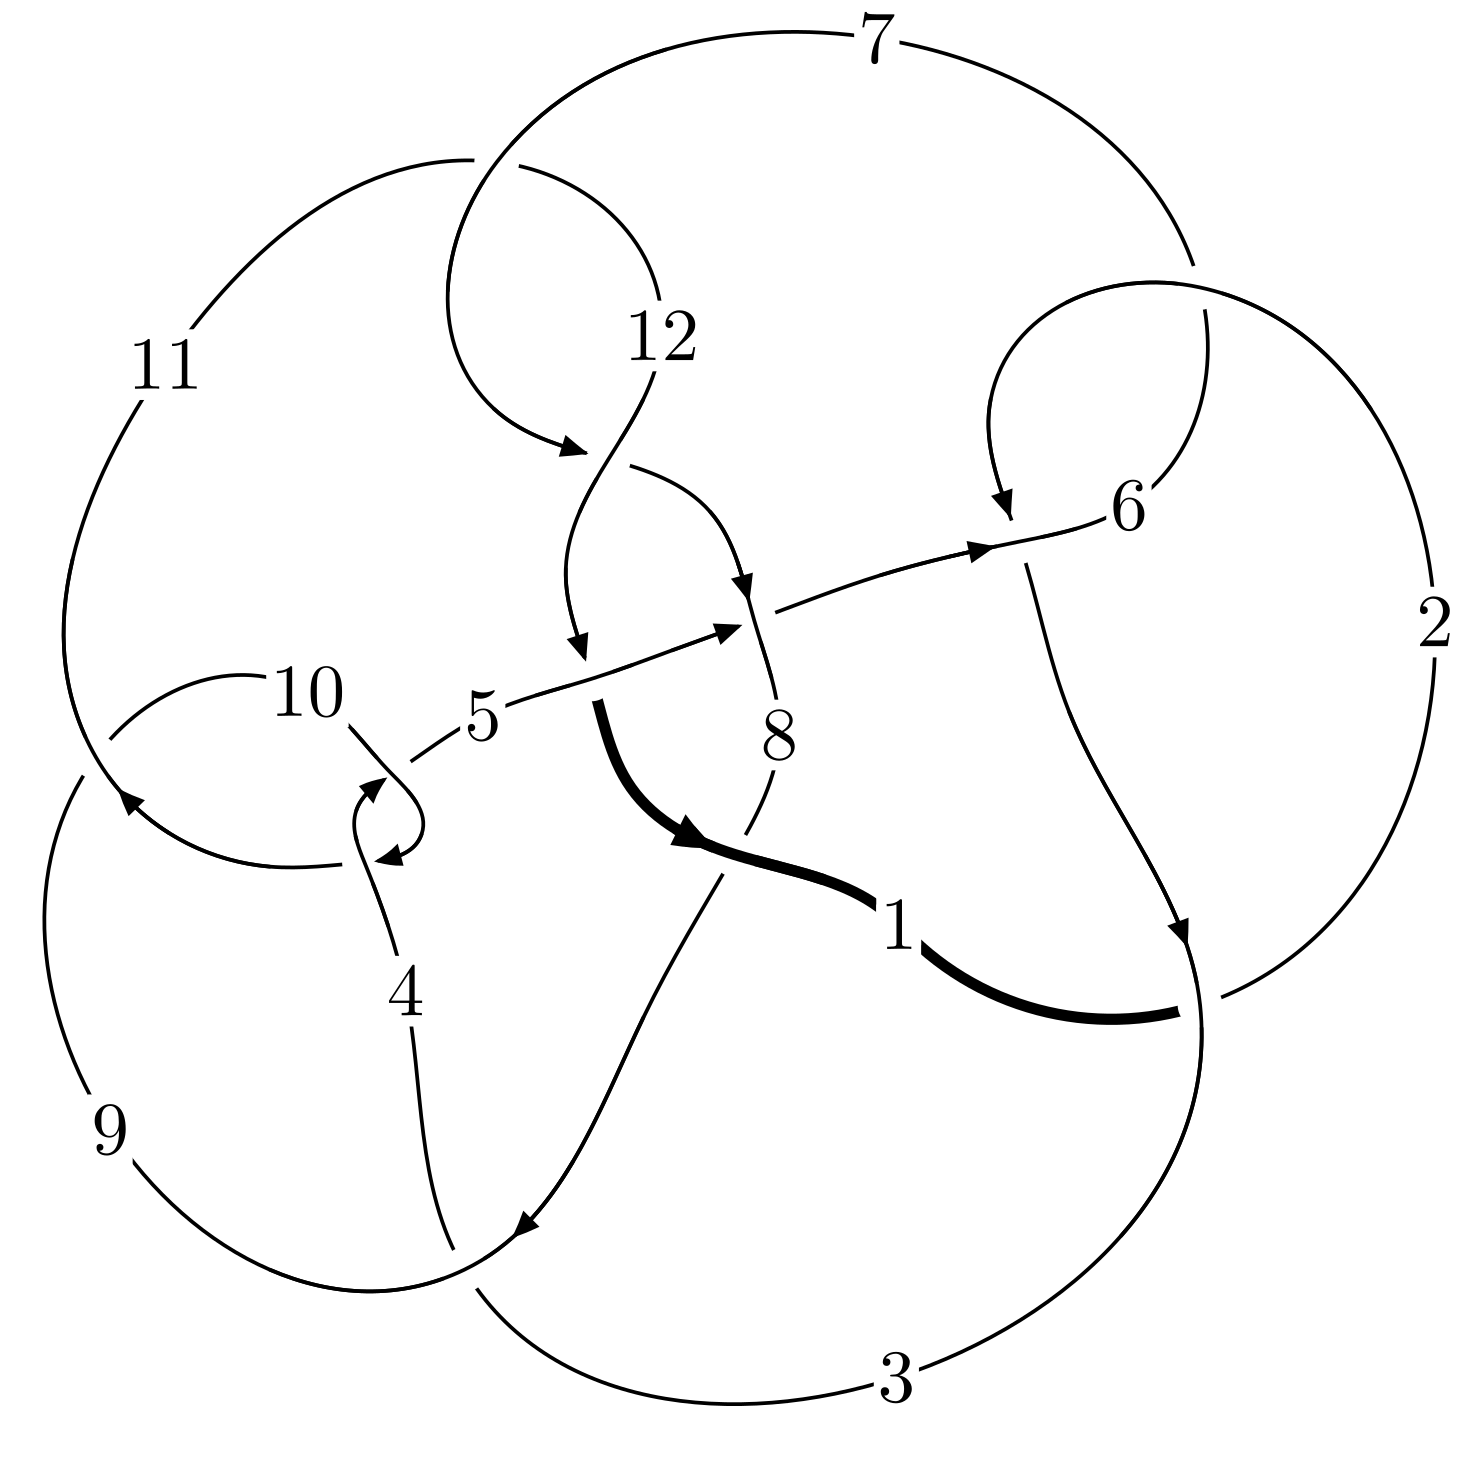
\includegraphics[width=112pt]{../../../GIT/diagram.site/Diagrams/png/1189_12a_0388.png}\\
\ \ \ A knot diagram\footnotemark}&
\allowdisplaybreaks
\textbf{Linearized knot diagam} \\
\cline{2-2}
 &
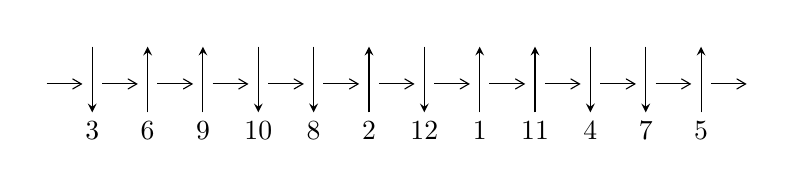
\begin{tikzpicture}[x=20pt, y=17pt]
	% nodes
	\node (C0) at (0, 0) {};
	\node (C1) at (1, 0) {};
	\node (C1U) at (1, +1) {};
	\node (C1D) at (1, -1) {3};

	\node (C2) at (2, 0) {};
	\node (C2U) at (2, +1) {};
	\node (C2D) at (2, -1) {6};

	\node (C3) at (3, 0) {};
	\node (C3U) at (3, +1) {};
	\node (C3D) at (3, -1) {9};

	\node (C4) at (4, 0) {};
	\node (C4U) at (4, +1) {};
	\node (C4D) at (4, -1) {10};

	\node (C5) at (5, 0) {};
	\node (C5U) at (5, +1) {};
	\node (C5D) at (5, -1) {8};

	\node (C6) at (6, 0) {};
	\node (C6U) at (6, +1) {};
	\node (C6D) at (6, -1) {2};

	\node (C7) at (7, 0) {};
	\node (C7U) at (7, +1) {};
	\node (C7D) at (7, -1) {12};

	\node (C8) at (8, 0) {};
	\node (C8U) at (8, +1) {};
	\node (C8D) at (8, -1) {1};

	\node (C9) at (9, 0) {};
	\node (C9U) at (9, +1) {};
	\node (C9D) at (9, -1) {11};

	\node (C10) at (10, 0) {};
	\node (C10U) at (10, +1) {};
	\node (C10D) at (10, -1) {4};

	\node (C11) at (11, 0) {};
	\node (C11U) at (11, +1) {};
	\node (C11D) at (11, -1) {7};

	\node (C12) at (12, 0) {};
	\node (C12U) at (12, +1) {};
	\node (C12D) at (12, -1) {5};
	\node (C13) at (13, 0) {};

	% arrows
	\draw[->,>={angle 60}]
	(C0) edge (C1) (C1) edge (C2) (C2) edge (C3) (C3) edge (C4) (C4) edge (C5) (C5) edge (C6) (C6) edge (C7) (C7) edge (C8) (C8) edge (C9) (C9) edge (C10) (C10) edge (C11) (C11) edge (C12) (C12) edge (C13) ;	\draw[->,>=stealth]
	(C1U) edge (C1D) (C2D) edge (C2U) (C3D) edge (C3U) (C4U) edge (C4D) (C5U) edge (C5D) (C6D) edge (C6U) (C7U) edge (C7D) (C8D) edge (C8U) (C9D) edge (C9U) (C10U) edge (C10D) (C11U) edge (C11D) (C12D) edge (C12U) ;
	\end{tikzpicture} \\
\hhline{~~} \\& 
\textbf{Solving Sequence} \\ \cline{2-2} 
 &
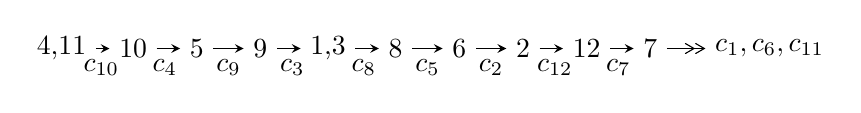
\begin{tikzpicture}[x=23pt, y=7pt]
	% node
	\node (A0) at (-1/8, 0) {4,11};
	\node (A1) at (1, 0) {10};
	\node (A2) at (2, 0) {5};
	\node (A3) at (3, 0) {9};
	\node (A4) at (65/16, 0) {1,3};
	\node (A5) at (41/8, 0) {8};
	\node (A6) at (49/8, 0) {6};
	\node (A7) at (57/8, 0) {2};
	\node (A8) at (65/8, 0) {12};
	\node (A9) at (73/8, 0) {7};
	\node (C1) at (1/2, -1) {$c_{10}$};
	\node (C2) at (3/2, -1) {$c_{4}$};
	\node (C3) at (5/2, -1) {$c_{9}$};
	\node (C4) at (7/2, -1) {$c_{3}$};
	\node (C5) at (37/8, -1) {$c_{8}$};
	\node (C6) at (45/8, -1) {$c_{5}$};
	\node (C7) at (53/8, -1) {$c_{2}$};
	\node (C8) at (61/8, -1) {$c_{12}$};
	\node (C9) at (69/8, -1) {$c_{7}$};
	\node (A10) at (11, 0) {$c_{1},c_{6},c_{11}$};

	% edge
	\draw[->,>=stealth]	
	(A0) edge (A1) (A1) edge (A2) (A2) edge (A3) (A3) edge (A4) (A4) edge (A5) (A5) edge (A6) (A6) edge (A7) (A7) edge (A8) (A8) edge (A9) ;
	\draw[->>,>={angle 60}]	
	(A9) edge (A10);
\end{tikzpicture} \\ 

\end{tabular} \\

\footnotetext{
The image of knot diagram is generated by the software ``\textbf{Draw programme}" developed by Andrew Bartholomew(\url{http://www.layer8.co.uk/maths/draw/index.htm\#Running-draw}), where we modified some parts for our purpose(\url{https://github.com/CATsTAILs/LinksPainter}).
}\phantom \\ \newline 
\centering \textbf{Ideals for irreducible components\footnotemark of $X_{\text{par}}$} 
 
\begin{align*}
I^u_{1}&=\langle 
1.10245\times10^{200} u^{137}-2.70350\times10^{199} u^{136}+\cdots+2.26798\times10^{199} b-2.98834\times10^{200},\\
\phantom{I^u_{1}}&\phantom{= \langle  }-2.02152\times10^{201} u^{137}-2.45020\times10^{201} u^{136}+\cdots+1.13399\times10^{200} a-5.74431\times10^{201},\\
\phantom{I^u_{1}}&\phantom{= \langle  }u^{138}+u^{137}+\cdots+2 u+1\rangle \\
I^u_{2}&=\langle 
u^{28}+4 u^{26}+\cdots+b-6,\;-9 u^{28}-67 u^{26}+\cdots+a-13,\;u^{30}+8 u^{28}+\cdots+6 u^2+1\rangle \\
I^u_{3}&=\langle 
u^2+b,\;a-1,\;u^{12}- u^{11}+2 u^{10}- u^9+u^7-3 u^6+3 u^5-2 u^4+2 u^2-2 u+1\rangle \\
I^u_{4}&=\langle 
b- u-1,\;a-1,\;u^2+u+1\rangle \\
\\
\end{align*}
\raggedright * 4 irreducible components of $\dim_{\mathbb{C}}=0$, with total 182 representations.\\
\footnotetext{All coefficients of polynomials are rational numbers. But the coefficients are sometimes approximated in decimal forms when there is not enough margin.}
\newpage
\renewcommand{\arraystretch}{1}
\centering \section*{I. $I^u_{1}= \langle 1.10\times10^{200} u^{137}-2.70\times10^{199} u^{136}+\cdots+2.27\times10^{199} b-2.99\times10^{200},\;-2.02\times10^{201} u^{137}-2.45\times10^{201} u^{136}+\cdots+1.13\times10^{200} a-5.74\times10^{201},\;u^{138}+u^{137}+\cdots+2 u+1 \rangle$}
\flushleft \textbf{(i) Arc colorings}\\
\begin{tabular}{m{7pt} m{180pt} m{7pt} m{180pt} }
\flushright $a_{4}=$&$\begin{pmatrix}0\\u\end{pmatrix}$ \\
\flushright $a_{11}=$&$\begin{pmatrix}1\\0\end{pmatrix}$ \\
\flushright $a_{10}=$&$\begin{pmatrix}1\\- u^2\end{pmatrix}$ \\
\flushright $a_{5}=$&$\begin{pmatrix}- u\\u^3+u\end{pmatrix}$ \\
\flushright $a_{9}=$&$\begin{pmatrix}u^2+1\\- u^2\end{pmatrix}$ \\
\flushright $a_{1}=$&$\begin{pmatrix}17.8266 u^{137}+21.6069 u^{136}+\cdots+72.5125 u+50.6558\\-4.86092 u^{137}+1.19203 u^{136}+\cdots-22.3388 u+13.1762\end{pmatrix}$ \\
\flushright $a_{3}=$&$\begin{pmatrix}- u^5-2 u^3- u\\u^5+u^3+u\end{pmatrix}$ \\
\flushright $a_{8}=$&$\begin{pmatrix}7.31158 u^{137}+10.8364 u^{136}+\cdots+42.2872 u+21.2695\\-11.0373 u^{137}-10.6810 u^{136}+\cdots-47.1603 u-19.8102\end{pmatrix}$ \\
\flushright $a_{6}=$&$\begin{pmatrix}15.0024 u^{137}+5.16035 u^{136}+\cdots+39.1591 u-6.06825\\4.75355 u^{137}+8.15710 u^{136}+\cdots+22.1169 u+23.1999\end{pmatrix}$ \\
\flushright $a_{2}=$&$\begin{pmatrix}21.6197 u^{137}+26.0663 u^{136}+\cdots+86.8487 u+61.5268\\-9.77139 u^{137}-3.70248 u^{136}+\cdots-41.5049 u+3.02636\end{pmatrix}$ \\
\flushright $a_{12}=$&$\begin{pmatrix}25.2621 u^{137}+27.9992 u^{136}+\cdots+102.662 u+62.2454\\-11.1523 u^{137}-4.87631 u^{136}+\cdots-47.1386 u+0.543510\end{pmatrix}$ \\
\flushright $a_{7}=$&$\begin{pmatrix}10.2508 u^{137}+17.9698 u^{136}+\cdots+70.9462 u+35.0066\\-0.698140 u^{137}-6.12399 u^{136}+\cdots-5.26299 u-19.2641\end{pmatrix}$\\&\end{tabular}
\flushleft \textbf{(ii) Obstruction class $= -1$}\\~\\
\flushleft \textbf{(iii) Cusp Shapes $= 1.31574 u^{137}-10.1454 u^{136}+\cdots-6.22611 u-51.1687$}\\~\\
\newpage\renewcommand{\arraystretch}{1}
\flushleft \textbf{(iv) u-Polynomials at the component}\newline \\
\begin{tabular}{m{50pt}|m{274pt}}
Crossings & \hspace{64pt}u-Polynomials at each crossing \\
\hline $$\begin{aligned}c_{1}\end{aligned}$$&$\begin{aligned}
&u^{138}+57 u^{137}+\cdots+4078944 u+222784
\end{aligned}$\\
\hline $$\begin{aligned}c_{2},c_{6}\end{aligned}$$&$\begin{aligned}
&u^{138}+7 u^{137}+\cdots+976 u+472
\end{aligned}$\\
\hline $$\begin{aligned}c_{3}\end{aligned}$$&$\begin{aligned}
&u^{138}+u^{137}+\cdots+1500 u+84625
\end{aligned}$\\
\hline $$\begin{aligned}c_{4},c_{10}\end{aligned}$$&$\begin{aligned}
&u^{138}- u^{137}+\cdots-2 u+1
\end{aligned}$\\
\hline $$\begin{aligned}c_{5}\end{aligned}$$&$\begin{aligned}
&u^{138}-4 u^{137}+\cdots-50 u+1
\end{aligned}$\\
\hline $$\begin{aligned}c_{7},c_{11}\end{aligned}$$&$\begin{aligned}
&u^{138}+3 u^{137}+\cdots+32098 u+2479
\end{aligned}$\\
\hline $$\begin{aligned}c_{8}\end{aligned}$$&$\begin{aligned}
&u^{138}- u^{137}+\cdots-312712 u+21829
\end{aligned}$\\
\hline $$\begin{aligned}c_{9}\end{aligned}$$&$\begin{aligned}
&u^{138}-73 u^{137}+\cdots-12 u+1
\end{aligned}$\\
\hline $$\begin{aligned}c_{12}\end{aligned}$$&$\begin{aligned}
&u^{138}-3 u^{137}+\cdots+126 u+107
\end{aligned}$\\
\hline
\end{tabular}\\~\\
\newpage\renewcommand{\arraystretch}{1}
\flushleft \textbf{(v) Riley Polynomials at the component}\newline \\
\begin{tabular}{m{50pt}|m{274pt}}
Crossings & \hspace{64pt}Riley Polynomials at each crossing \\
\hline $$\begin{aligned}c_{1}\end{aligned}$$&$\begin{aligned}
&y^{138}+57 y^{137}+\cdots+592047023616 y+49632710656
\end{aligned}$\\
\hline $$\begin{aligned}c_{2},c_{6}\end{aligned}$$&$\begin{aligned}
&y^{138}+57 y^{137}+\cdots+4078944 y+222784
\end{aligned}$\\
\hline $$\begin{aligned}c_{3}\end{aligned}$$&$\begin{aligned}
&y^{138}-63 y^{137}+\cdots+1166513601250 y+7161390625
\end{aligned}$\\
\hline $$\begin{aligned}c_{4},c_{10}\end{aligned}$$&$\begin{aligned}
&y^{138}+73 y^{137}+\cdots+12 y+1
\end{aligned}$\\
\hline $$\begin{aligned}c_{5}\end{aligned}$$&$\begin{aligned}
&y^{138}-6 y^{137}+\cdots-84 y+1
\end{aligned}$\\
\hline $$\begin{aligned}c_{7},c_{11}\end{aligned}$$&$\begin{aligned}
&y^{138}-89 y^{137}+\cdots-992898284 y+6145441
\end{aligned}$\\
\hline $$\begin{aligned}c_{8}\end{aligned}$$&$\begin{aligned}
&y^{138}-33 y^{137}+\cdots-25000518340 y+476505241
\end{aligned}$\\
\hline $$\begin{aligned}c_{9}\end{aligned}$$&$\begin{aligned}
&y^{138}+5 y^{137}+\cdots+56 y+1
\end{aligned}$\\
\hline $$\begin{aligned}c_{12}\end{aligned}$$&$\begin{aligned}
&y^{138}+13 y^{137}+\cdots+1100348 y+11449
\end{aligned}$\\
\hline
\end{tabular}\\~\\
\newpage\flushleft \textbf{(vi) Complex Volumes and Cusp Shapes}
$$\begin{array}{c|c|c}  
\text{Solutions to }I^u_{1}& \I (\text{vol} + \sqrt{-1}CS) & \text{Cusp shape}\\
 \hline 
\begin{aligned}
u &= -0.748280 + 0.644042 I \\
a &= -0.610770 - 0.383166 I \\
b &= \phantom{-}0.279919 + 0.054730 I\end{aligned}
 & -3.23015 - 1.44711 I & \phantom{-0.000000 } 0 \\ \hline\begin{aligned}
u &= -0.748280 - 0.644042 I \\
a &= -0.610770 + 0.383166 I \\
b &= \phantom{-}0.279919 - 0.054730 I\end{aligned}
 & -3.23015 + 1.44711 I & \phantom{-0.000000 } 0 \\ \hline\begin{aligned}
u &= -0.932996 + 0.397354 I \\
a &= -0.560435 - 0.059752 I \\
b &= \phantom{-}0.675164 - 0.194043 I\end{aligned}
 & -0.20912 - 4.87826 I & \phantom{-0.000000 } 0 \\ \hline\begin{aligned}
u &= -0.932996 - 0.397354 I \\
a &= -0.560435 + 0.059752 I \\
b &= \phantom{-}0.675164 + 0.194043 I\end{aligned}
 & -0.20912 + 4.87826 I & \phantom{-0.000000 } 0 \\ \hline\begin{aligned}
u &= -0.639139 + 0.717002 I \\
a &= -0.526322 - 0.610491 I \\
b &= \phantom{-}0.065518 + 0.290224 I\end{aligned}
 & -3.14704 - 1.39877 I & \phantom{-0.000000 } 0 \\ \hline\begin{aligned}
u &= -0.639139 - 0.717002 I \\
a &= -0.526322 + 0.610491 I \\
b &= \phantom{-}0.065518 - 0.290224 I\end{aligned}
 & -3.14704 + 1.39877 I & \phantom{-0.000000 } 0 \\ \hline\begin{aligned}
u &= \phantom{-}0.507689 + 0.814153 I \\
a &= \phantom{-}0.460248 - 0.369612 I \\
b &= -0.259173 + 0.658419 I\end{aligned}
 & \phantom{-}0.62104 - 2.03888 I & \phantom{-0.000000 } 0 \\ \hline\begin{aligned}
u &= \phantom{-}0.507689 - 0.814153 I \\
a &= \phantom{-}0.460248 + 0.369612 I \\
b &= -0.259173 - 0.658419 I\end{aligned}
 & \phantom{-}0.62104 + 2.03888 I & \phantom{-0.000000 } 0 \\ \hline\begin{aligned}
u &= -0.657750 + 0.812749 I \\
a &= -0.759257 + 0.080546 I \\
b &= \phantom{-}0.147457 + 0.240247 I\end{aligned}
 & -2.90258 + 6.42158 I & \phantom{-0.000000 } 0 \\ \hline\begin{aligned}
u &= -0.657750 - 0.812749 I \\
a &= -0.759257 - 0.080546 I \\
b &= \phantom{-}0.147457 - 0.240247 I\end{aligned}
 & -2.90258 - 6.42158 I & \phantom{-0.000000 } 0\\
 \hline 
 \end{array}$$\newpage$$\begin{array}{c|c|c}  
\text{Solutions to }I^u_{1}& \I (\text{vol} + \sqrt{-1}CS) & \text{Cusp shape}\\
 \hline 
\begin{aligned}
u &= \phantom{-}0.900380 + 0.306762 I \\
a &= -0.533987 - 0.027012 I \\
b &= \phantom{-}0.675781 + 0.175122 I\end{aligned}
 & \phantom{-}0.319495 - 0.269839 I & \phantom{-0.000000 } 0 \\ \hline\begin{aligned}
u &= \phantom{-}0.900380 - 0.306762 I \\
a &= -0.533987 + 0.027012 I \\
b &= \phantom{-}0.675781 - 0.175122 I\end{aligned}
 & \phantom{-}0.319495 + 0.269839 I & \phantom{-0.000000 } 0 \\ \hline\begin{aligned}
u &= -0.505496 + 0.784641 I \\
a &= \phantom{-}0.155415 - 0.211164 I \\
b &= \phantom{-}0.813512 - 0.448155 I\end{aligned}
 & -3.41327 + 2.08249 I & \phantom{-0.000000 } 0 \\ \hline\begin{aligned}
u &= -0.505496 - 0.784641 I \\
a &= \phantom{-}0.155415 + 0.211164 I \\
b &= \phantom{-}0.813512 + 0.448155 I\end{aligned}
 & -3.41327 - 2.08249 I & \phantom{-0.000000 } 0 \\ \hline\begin{aligned}
u &= -0.002295 + 0.933167 I \\
a &= \phantom{-}0.348407 - 1.168260 I \\
b &= \phantom{-}1.02831 + 1.09047 I\end{aligned}
 & -2.58537 - 3.57558 I & \phantom{-0.000000 } 0 \\ \hline\begin{aligned}
u &= -0.002295 - 0.933167 I \\
a &= \phantom{-}0.348407 + 1.168260 I \\
b &= \phantom{-}1.02831 - 1.09047 I\end{aligned}
 & -2.58537 + 3.57558 I & \phantom{-0.000000 } 0 \\ \hline\begin{aligned}
u &= -0.586344 + 0.712656 I \\
a &= \phantom{-}0.256709 + 0.327840 I \\
b &= -0.216062 - 1.112430 I\end{aligned}
 & -0.42447 + 6.42817 I & \phantom{-0.000000 } 0 \\ \hline\begin{aligned}
u &= -0.586344 - 0.712656 I \\
a &= \phantom{-}0.256709 - 0.327840 I \\
b &= -0.216062 + 1.112430 I\end{aligned}
 & -0.42447 - 6.42817 I & \phantom{-0.000000 } 0 \\ \hline\begin{aligned}
u &= -0.876763 + 0.277742 I \\
a &= -2.01971 + 0.48046 I \\
b &= \phantom{-}1.70197 - 0.89884 I\end{aligned}
 & -1.8751 - 14.3871 I & \phantom{-0.000000 } 0 \\ \hline\begin{aligned}
u &= -0.876763 - 0.277742 I \\
a &= -2.01971 - 0.48046 I \\
b &= \phantom{-}1.70197 + 0.89884 I\end{aligned}
 & -1.8751 + 14.3871 I & \phantom{-0.000000 } 0\\
 \hline 
 \end{array}$$\newpage$$\begin{array}{c|c|c}  
\text{Solutions to }I^u_{1}& \I (\text{vol} + \sqrt{-1}CS) & \text{Cusp shape}\\
 \hline 
\begin{aligned}
u &= \phantom{-}0.675148 + 0.623419 I \\
a &= -0.628890 - 0.768440 I \\
b &= -0.218688 - 0.249187 I\end{aligned}
 & -7.79238 - 3.57360 I & \phantom{-0.000000 } 0 \\ \hline\begin{aligned}
u &= \phantom{-}0.675148 - 0.623419 I \\
a &= -0.628890 + 0.768440 I \\
b &= -0.218688 + 0.249187 I\end{aligned}
 & -7.79238 + 3.57360 I & \phantom{-0.000000 } 0 \\ \hline\begin{aligned}
u &= -0.308930 + 1.036300 I \\
a &= -0.26750 - 1.81985 I \\
b &= \phantom{-}2.33740 + 0.80264 I\end{aligned}
 & -2.46898 - 3.18569 I & \phantom{-0.000000 } 0 \\ \hline\begin{aligned}
u &= -0.308930 - 1.036300 I \\
a &= -0.26750 + 1.81985 I \\
b &= \phantom{-}2.33740 - 0.80264 I\end{aligned}
 & -2.46898 + 3.18569 I & \phantom{-0.000000 } 0 \\ \hline\begin{aligned}
u &= \phantom{-}0.351642 + 0.833956 I \\
a &= \phantom{-}0.842916 - 0.075164 I \\
b &= \phantom{-}0.141774 - 0.101162 I\end{aligned}
 & \phantom{-}0.32671 - 1.54792 I & \phantom{-0.000000 } 0 \\ \hline\begin{aligned}
u &= \phantom{-}0.351642 - 0.833956 I \\
a &= \phantom{-}0.842916 + 0.075164 I \\
b &= \phantom{-}0.141774 + 0.101162 I\end{aligned}
 & \phantom{-}0.32671 + 1.54792 I & \phantom{-0.000000 } 0 \\ \hline\begin{aligned}
u &= \phantom{-}0.762004 + 0.807024 I \\
a &= -0.441904 - 0.113955 I \\
b &= \phantom{-}0.141367 - 0.472899 I\end{aligned}
 & -5.04826 - 11.36710 I & \phantom{-0.000000 } 0 \\ \hline\begin{aligned}
u &= \phantom{-}0.762004 - 0.807024 I \\
a &= -0.441904 + 0.113955 I \\
b &= \phantom{-}0.141367 + 0.472899 I\end{aligned}
 & -5.04826 + 11.36710 I & \phantom{-0.000000 } 0 \\ \hline\begin{aligned}
u &= -0.459758 + 1.015400 I \\
a &= \phantom{-}1.39876 - 2.58387 I \\
b &= \phantom{-}1.97149 + 1.80899 I\end{aligned}
 & -2.96281 - 1.00766 I & \phantom{-0.000000 } 0 \\ \hline\begin{aligned}
u &= -0.459758 - 1.015400 I \\
a &= \phantom{-}1.39876 + 2.58387 I \\
b &= \phantom{-}1.97149 - 1.80899 I\end{aligned}
 & -2.96281 + 1.00766 I & \phantom{-0.000000 } 0\\
 \hline 
 \end{array}$$\newpage$$\begin{array}{c|c|c}  
\text{Solutions to }I^u_{1}& \I (\text{vol} + \sqrt{-1}CS) & \text{Cusp shape}\\
 \hline 
\begin{aligned}
u &= \phantom{-}0.833669 + 0.246306 I \\
a &= -2.07608 - 0.62945 I \\
b &= \phantom{-}1.59871 + 0.86388 I\end{aligned}
 & \phantom{-}0.18672 + 8.44910 I & \phantom{-0.000000 } 0 \\ \hline\begin{aligned}
u &= \phantom{-}0.833669 - 0.246306 I \\
a &= -2.07608 + 0.62945 I \\
b &= \phantom{-}1.59871 - 0.86388 I\end{aligned}
 & \phantom{-}0.18672 - 8.44910 I & \phantom{-0.000000 } 0 \\ \hline\begin{aligned}
u &= \phantom{-}0.631156 + 0.942527 I \\
a &= \phantom{-}0.032130 + 0.523672 I \\
b &= -0.562343 - 0.343106 I\end{aligned}
 & -6.87135 - 1.44864 I & \phantom{-0.000000 } 0 \\ \hline\begin{aligned}
u &= \phantom{-}0.631156 - 0.942527 I \\
a &= \phantom{-}0.032130 - 0.523672 I \\
b &= -0.562343 + 0.343106 I\end{aligned}
 & -6.87135 + 1.44864 I & \phantom{-0.000000 } 0 \\ \hline\begin{aligned}
u &= -0.359853 + 0.779267 I \\
a &= -1.64500 - 1.09008 I \\
b &= \phantom{-}0.90099 - 1.77749 I\end{aligned}
 & -3.04538 + 5.83097 I & \phantom{-0.000000 } 0 \\ \hline\begin{aligned}
u &= -0.359853 - 0.779267 I \\
a &= -1.64500 + 1.09008 I \\
b &= \phantom{-}0.90099 + 1.77749 I\end{aligned}
 & -3.04538 - 5.83097 I & \phantom{-0.000000 } 0 \\ \hline\begin{aligned}
u &= \phantom{-}0.784849 + 0.833178 I \\
a &= -0.336576 + 0.331522 I \\
b &= -0.187643 + 0.128653 I\end{aligned}
 & -4.99993 + 5.64141 I & \phantom{-0.000000 } 0 \\ \hline\begin{aligned}
u &= \phantom{-}0.784849 - 0.833178 I \\
a &= -0.336576 - 0.331522 I \\
b &= -0.187643 - 0.128653 I\end{aligned}
 & -4.99993 - 5.64141 I & \phantom{-0.000000 } 0 \\ \hline\begin{aligned}
u &= \phantom{-}0.055678 + 0.850726 I \\
a &= \phantom{-}0.331880 + 0.528641 I \\
b &= \phantom{-}0.585870 + 0.867197 I\end{aligned}
 & \phantom{-}1.17077 - 1.75880 I & \phantom{-0.000000 } 0 \\ \hline\begin{aligned}
u &= \phantom{-}0.055678 - 0.850726 I \\
a &= \phantom{-}0.331880 - 0.528641 I \\
b &= \phantom{-}0.585870 - 0.867197 I\end{aligned}
 & \phantom{-}1.17077 + 1.75880 I & \phantom{-0.000000 } 0\\
 \hline 
 \end{array}$$\newpage$$\begin{array}{c|c|c}  
\text{Solutions to }I^u_{1}& \I (\text{vol} + \sqrt{-1}CS) & \text{Cusp shape}\\
 \hline 
\begin{aligned}
u &= \phantom{-}0.414877 + 1.070120 I \\
a &= \phantom{-}0.55316 - 1.36199 I \\
b &= -1.52236 + 0.17162 I\end{aligned}
 & \phantom{-}1.25960 - 1.39359 I & \phantom{-0.000000 } 0 \\ \hline\begin{aligned}
u &= \phantom{-}0.414877 - 1.070120 I \\
a &= \phantom{-}0.55316 + 1.36199 I \\
b &= -1.52236 - 0.17162 I\end{aligned}
 & \phantom{-}1.25960 + 1.39359 I & \phantom{-0.000000 } 0 \\ \hline\begin{aligned}
u &= -0.540226 + 1.032780 I \\
a &= -0.60369 - 2.18713 I \\
b &= \phantom{-}2.20825 - 0.06733 I\end{aligned}
 & -3.53762 + 6.87962 I & \phantom{-0.000000 } 0 \\ \hline\begin{aligned}
u &= -0.540226 - 1.032780 I \\
a &= -0.60369 + 2.18713 I \\
b &= \phantom{-}2.20825 + 0.06733 I\end{aligned}
 & -3.53762 - 6.87962 I & \phantom{-0.000000 } 0 \\ \hline\begin{aligned}
u &= -0.437879 + 1.081410 I \\
a &= \phantom{-}0.79631 - 1.65724 I \\
b &= \phantom{-}0.25068 + 1.53384 I\end{aligned}
 & \phantom{-}2.95472 + 0.07846 I & \phantom{-0.000000 } 0 \\ \hline\begin{aligned}
u &= -0.437879 - 1.081410 I \\
a &= \phantom{-}0.79631 + 1.65724 I \\
b &= \phantom{-}0.25068 - 1.53384 I\end{aligned}
 & \phantom{-}2.95472 - 0.07846 I & \phantom{-0.000000 } 0 \\ \hline\begin{aligned}
u &= \phantom{-}0.717790 + 0.415508 I \\
a &= -1.151190 + 0.406748 I \\
b &= \phantom{-}1.206330 - 0.686473 I\end{aligned}
 & -4.57232 - 0.12230 I & \phantom{-0.000000 } 0 \\ \hline\begin{aligned}
u &= \phantom{-}0.717790 - 0.415508 I \\
a &= -1.151190 - 0.406748 I \\
b &= \phantom{-}1.206330 + 0.686473 I\end{aligned}
 & -4.57232 + 0.12230 I & \phantom{-0.000000 } 0 \\ \hline\begin{aligned}
u &= \phantom{-}0.477056 + 1.070260 I \\
a &= \phantom{-}0.53665 + 1.77130 I \\
b &= \phantom{-}1.56832 - 0.83541 I\end{aligned}
 & \phantom{-}0.02851 - 3.36557 I & \phantom{-0.000000 } 0 \\ \hline\begin{aligned}
u &= \phantom{-}0.477056 - 1.070260 I \\
a &= \phantom{-}0.53665 - 1.77130 I \\
b &= \phantom{-}1.56832 + 0.83541 I\end{aligned}
 & \phantom{-}0.02851 + 3.36557 I & \phantom{-0.000000 } 0\\
 \hline 
 \end{array}$$\newpage$$\begin{array}{c|c|c}  
\text{Solutions to }I^u_{1}& \I (\text{vol} + \sqrt{-1}CS) & \text{Cusp shape}\\
 \hline 
\begin{aligned}
u &= -0.646252 + 0.512234 I \\
a &= -1.71957 - 0.10186 I \\
b &= \phantom{-}1.71208 - 0.29986 I\end{aligned}
 & -5.07463 - 2.23565 I & \phantom{-0.000000 } 0 \\ \hline\begin{aligned}
u &= -0.646252 - 0.512234 I \\
a &= -1.71957 + 0.10186 I \\
b &= \phantom{-}1.71208 + 0.29986 I\end{aligned}
 & -5.07463 + 2.23565 I & \phantom{-0.000000 } 0 \\ \hline\begin{aligned}
u &= -0.466150 + 1.083490 I \\
a &= -1.23938 - 0.94255 I \\
b &= \phantom{-}0.268720 - 0.691177 I\end{aligned}
 & -0.09519 + 5.03975 I & \phantom{-0.000000 } 0 \\ \hline\begin{aligned}
u &= -0.466150 - 1.083490 I \\
a &= -1.23938 + 0.94255 I \\
b &= \phantom{-}0.268720 + 0.691177 I\end{aligned}
 & -0.09519 - 5.03975 I & \phantom{-0.000000 } 0 \\ \hline\begin{aligned}
u &= \phantom{-}0.775971 + 0.259276 I \\
a &= \phantom{-}2.06204 + 0.43638 I \\
b &= -1.77887 - 0.94228 I\end{aligned}
 & \phantom{-}1.75979 + 7.99239 I & \phantom{-0.000000 } 0 \\ \hline\begin{aligned}
u &= \phantom{-}0.775971 - 0.259276 I \\
a &= \phantom{-}2.06204 - 0.43638 I \\
b &= -1.77887 + 0.94228 I\end{aligned}
 & \phantom{-}1.75979 - 7.99239 I & \phantom{-0.000000 } 0 \\ \hline\begin{aligned}
u &= -0.608762 + 1.020920 I \\
a &= -0.691827 - 0.686455 I \\
b &= \phantom{-}0.699993 - 0.018161 I\end{aligned}
 & -2.00844 + 6.60279 I & \phantom{-0.000000 } 0 \\ \hline\begin{aligned}
u &= -0.608762 - 1.020920 I \\
a &= -0.691827 + 0.686455 I \\
b &= \phantom{-}0.699993 + 0.018161 I\end{aligned}
 & -2.00844 - 6.60279 I & \phantom{-0.000000 } 0 \\ \hline\begin{aligned}
u &= -0.157115 + 1.183080 I \\
a &= \phantom{-}0.546397 - 0.569497 I \\
b &= \phantom{-}0.424413 + 0.447750 I\end{aligned}
 & \phantom{-}5.45597 - 2.08589 I & \phantom{-0.000000 } 0 \\ \hline\begin{aligned}
u &= -0.157115 - 1.183080 I \\
a &= \phantom{-}0.546397 + 0.569497 I \\
b &= \phantom{-}0.424413 - 0.447750 I\end{aligned}
 & \phantom{-}5.45597 + 2.08589 I & \phantom{-0.000000 } 0\\
 \hline 
 \end{array}$$\newpage$$\begin{array}{c|c|c}  
\text{Solutions to }I^u_{1}& \I (\text{vol} + \sqrt{-1}CS) & \text{Cusp shape}\\
 \hline 
\begin{aligned}
u &= -0.481072 + 1.093010 I \\
a &= -0.697789 - 0.457258 I \\
b &= \phantom{-}1.79379 - 0.78867 I\end{aligned}
 & \phantom{-}2.62273 + 7.06472 I & \phantom{-0.000000 } 0 \\ \hline\begin{aligned}
u &= -0.481072 - 1.093010 I \\
a &= -0.697789 + 0.457258 I \\
b &= \phantom{-}1.79379 + 0.78867 I\end{aligned}
 & \phantom{-}2.62273 - 7.06472 I & \phantom{-0.000000 } 0 \\ \hline\begin{aligned}
u &= \phantom{-}0.426878 + 1.121990 I \\
a &= -0.869950 + 0.927785 I \\
b &= \phantom{-}2.29389 + 0.55773 I\end{aligned}
 & \phantom{-}4.24755 - 0.55395 I & \phantom{-0.000000 } 0 \\ \hline\begin{aligned}
u &= \phantom{-}0.426878 - 1.121990 I \\
a &= -0.869950 - 0.927785 I \\
b &= \phantom{-}2.29389 - 0.55773 I\end{aligned}
 & \phantom{-}4.24755 + 0.55395 I & \phantom{-0.000000 } 0 \\ \hline\begin{aligned}
u &= \phantom{-}0.482092 + 1.102240 I \\
a &= -0.73817 - 1.73876 I \\
b &= -1.75836 + 1.68519 I\end{aligned}
 & \phantom{-}0.73692 - 5.83263 I & \phantom{-0.000000 } 0 \\ \hline\begin{aligned}
u &= \phantom{-}0.482092 - 1.102240 I \\
a &= -0.73817 + 1.73876 I \\
b &= -1.75836 - 1.68519 I\end{aligned}
 & \phantom{-}0.73692 + 5.83263 I & \phantom{-0.000000 } 0 \\ \hline\begin{aligned}
u &= -0.722215 + 0.333026 I \\
a &= -2.60247 + 0.51955 I \\
b &= \phantom{-}1.43509 - 1.10683 I\end{aligned}
 & -6.52298 - 5.63767 I & -6.96561 + 5.54235 I \\ \hline\begin{aligned}
u &= -0.722215 - 0.333026 I \\
a &= -2.60247 - 0.51955 I \\
b &= \phantom{-}1.43509 + 1.10683 I\end{aligned}
 & -6.52298 + 5.63767 I & -6.96561 - 5.54235 I \\ \hline\begin{aligned}
u &= \phantom{-}0.224822 + 1.184760 I \\
a &= \phantom{-}0.639971 + 0.617614 I \\
b &= \phantom{-}0.537226 - 0.485258 I\end{aligned}
 & \phantom{-}5.44782 - 3.44229 I & \phantom{-0.000000 } 0 \\ \hline\begin{aligned}
u &= \phantom{-}0.224822 - 1.184760 I \\
a &= \phantom{-}0.639971 - 0.617614 I \\
b &= \phantom{-}0.537226 + 0.485258 I\end{aligned}
 & \phantom{-}5.44782 + 3.44229 I & \phantom{-0.000000 } 0\\
 \hline 
 \end{array}$$\newpage$$\begin{array}{c|c|c}  
\text{Solutions to }I^u_{1}& \I (\text{vol} + \sqrt{-1}CS) & \text{Cusp shape}\\
 \hline 
\begin{aligned}
u &= \phantom{-}0.294523 + 1.173140 I \\
a &= \phantom{-}0.02129 - 1.59871 I \\
b &= -1.75952 + 0.05382 I\end{aligned}
 & \phantom{-}6.12367 + 4.70777 I & \phantom{-0.000000 } 0 \\ \hline\begin{aligned}
u &= \phantom{-}0.294523 - 1.173140 I \\
a &= \phantom{-}0.02129 + 1.59871 I \\
b &= -1.75952 - 0.05382 I\end{aligned}
 & \phantom{-}6.12367 - 4.70777 I & \phantom{-0.000000 } 0 \\ \hline\begin{aligned}
u &= -0.766583 + 0.191365 I \\
a &= \phantom{-}1.95474 - 0.48334 I \\
b &= -1.60377 + 0.72697 I\end{aligned}
 & \phantom{-}3.31803 - 2.71598 I & \phantom{-}2.61257 + 1.91367 I \\ \hline\begin{aligned}
u &= -0.766583 - 0.191365 I \\
a &= \phantom{-}1.95474 + 0.48334 I \\
b &= -1.60377 - 0.72697 I\end{aligned}
 & \phantom{-}3.31803 + 2.71598 I & \phantom{-}2.61257 - 1.91367 I \\ \hline\begin{aligned}
u &= \phantom{-}0.468517 + 1.121520 I \\
a &= \phantom{-}0.73584 + 2.02735 I \\
b &= \phantom{-}1.05117 - 1.85791 I\end{aligned}
 & \phantom{-}3.95618 - 7.12231 I & \phantom{-0.000000 } 0 \\ \hline\begin{aligned}
u &= \phantom{-}0.468517 - 1.121520 I \\
a &= \phantom{-}0.73584 - 2.02735 I \\
b &= \phantom{-}1.05117 + 1.85791 I\end{aligned}
 & \phantom{-}3.95618 + 7.12231 I & \phantom{-0.000000 } 0 \\ \hline\begin{aligned}
u &= \phantom{-}0.576038 + 1.083480 I \\
a &= -1.07623 + 1.16309 I \\
b &= \phantom{-}1.017400 + 0.804040 I\end{aligned}
 & -2.61627 - 4.82946 I & \phantom{-0.000000 } 0 \\ \hline\begin{aligned}
u &= \phantom{-}0.576038 - 1.083480 I \\
a &= -1.07623 - 1.16309 I \\
b &= \phantom{-}1.017400 - 0.804040 I\end{aligned}
 & -2.61627 + 4.82946 I & \phantom{-0.000000 } 0 \\ \hline\begin{aligned}
u &= -0.340294 + 1.182050 I \\
a &= \phantom{-}0.11787 + 1.48216 I \\
b &= -1.81420 - 0.09781 I\end{aligned}
 & \phantom{-}7.41416 + 0.88258 I & \phantom{-0.000000 } 0 \\ \hline\begin{aligned}
u &= -0.340294 - 1.182050 I \\
a &= \phantom{-}0.11787 - 1.48216 I \\
b &= -1.81420 + 0.09781 I\end{aligned}
 & \phantom{-}7.41416 - 0.88258 I & \phantom{-0.000000 } 0\\
 \hline 
 \end{array}$$\newpage$$\begin{array}{c|c|c}  
\text{Solutions to }I^u_{1}& \I (\text{vol} + \sqrt{-1}CS) & \text{Cusp shape}\\
 \hline 
\begin{aligned}
u &= \phantom{-}0.502474 + 1.125750 I \\
a &= -1.20050 + 1.00972 I \\
b &= \phantom{-}0.396619 + 0.918271 I\end{aligned}
 & -0.86260 - 9.72934 I & \phantom{-0.000000 } 0 \\ \hline\begin{aligned}
u &= \phantom{-}0.502474 - 1.125750 I \\
a &= -1.20050 - 1.00972 I \\
b &= \phantom{-}0.396619 - 0.918271 I\end{aligned}
 & -0.86260 + 9.72934 I & \phantom{-0.000000 } 0 \\ \hline\begin{aligned}
u &= \phantom{-}0.386148 + 1.172850 I \\
a &= -0.35243 - 1.62014 I \\
b &= -0.77820 + 1.44305 I\end{aligned}
 & \phantom{-}2.87431 + 1.77348 I & \phantom{-0.000000 } 0 \\ \hline\begin{aligned}
u &= \phantom{-}0.386148 - 1.172850 I \\
a &= -0.35243 + 1.62014 I \\
b &= -0.77820 - 1.44305 I\end{aligned}
 & \phantom{-}2.87431 - 1.77348 I & \phantom{-0.000000 } 0 \\ \hline\begin{aligned}
u &= -0.547313 + 1.117630 I \\
a &= \phantom{-}0.13739 - 2.31147 I \\
b &= \phantom{-}2.28237 + 1.68690 I\end{aligned}
 & -4.22099 + 10.47690 I & \phantom{-0.000000 } 0 \\ \hline\begin{aligned}
u &= -0.547313 - 1.117630 I \\
a &= \phantom{-}0.13739 + 2.31147 I \\
b &= \phantom{-}2.28237 - 1.68690 I\end{aligned}
 & -4.22099 - 10.47690 I & \phantom{-0.000000 } 0 \\ \hline\begin{aligned}
u &= -0.449881 + 1.169470 I \\
a &= \phantom{-}0.36792 + 1.45628 I \\
b &= -2.09251 - 0.54636 I\end{aligned}
 & \phantom{-}5.41259 + 4.06951 I & \phantom{-0.000000 } 0 \\ \hline\begin{aligned}
u &= -0.449881 - 1.169470 I \\
a &= \phantom{-}0.36792 - 1.45628 I \\
b &= -2.09251 + 0.54636 I\end{aligned}
 & \phantom{-}5.41259 - 4.06951 I & \phantom{-0.000000 } 0 \\ \hline\begin{aligned}
u &= \phantom{-}0.285497 + 1.221200 I \\
a &= -0.230904 + 1.209670 I \\
b &= \phantom{-}1.80867 - 0.03426 I\end{aligned}
 & \phantom{-}4.83744 + 4.88572 I & \phantom{-0.000000 } 0 \\ \hline\begin{aligned}
u &= \phantom{-}0.285497 - 1.221200 I \\
a &= -0.230904 - 1.209670 I \\
b &= \phantom{-}1.80867 + 0.03426 I\end{aligned}
 & \phantom{-}4.83744 - 4.88572 I & \phantom{-0.000000 } 0\\
 \hline 
 \end{array}$$\newpage$$\begin{array}{c|c|c}  
\text{Solutions to }I^u_{1}& \I (\text{vol} + \sqrt{-1}CS) & \text{Cusp shape}\\
 \hline 
\begin{aligned}
u &= \phantom{-}0.730810 + 0.132013 I \\
a &= \phantom{-}1.87462 - 1.41487 I \\
b &= -1.236480 + 0.030970 I\end{aligned}
 & -0.86799 + 5.55501 I & -2.80187 - 9.67670 I \\ \hline\begin{aligned}
u &= \phantom{-}0.730810 - 0.132013 I \\
a &= \phantom{-}1.87462 + 1.41487 I \\
b &= -1.236480 - 0.030970 I\end{aligned}
 & -0.86799 - 5.55501 I & -2.80187 + 9.67670 I \\ \hline\begin{aligned}
u &= -0.448095 + 1.174840 I \\
a &= -0.03447 + 1.70384 I \\
b &= -1.71767 - 1.10560 I\end{aligned}
 & \phantom{-}5.42668 + 4.33154 I & \phantom{-0.000000 } 0 \\ \hline\begin{aligned}
u &= -0.448095 - 1.174840 I \\
a &= -0.03447 - 1.70384 I \\
b &= -1.71767 + 1.10560 I\end{aligned}
 & \phantom{-}5.42668 - 4.33154 I & \phantom{-0.000000 } 0 \\ \hline\begin{aligned}
u &= \phantom{-}0.497105 + 1.165690 I \\
a &= \phantom{-}0.925864 - 1.025280 I \\
b &= -2.50249 - 0.12633 I\end{aligned}
 & \phantom{-}2.09741 - 10.13010 I & \phantom{-0.000000 } 0 \\ \hline\begin{aligned}
u &= \phantom{-}0.497105 - 1.165690 I \\
a &= \phantom{-}0.925864 + 1.025280 I \\
b &= -2.50249 + 0.12633 I\end{aligned}
 & \phantom{-}2.09741 + 10.13010 I & \phantom{-0.000000 } 0 \\ \hline\begin{aligned}
u &= -0.522583 + 1.164700 I \\
a &= -0.22839 + 1.93063 I \\
b &= -2.13174 - 1.04573 I\end{aligned}
 & \phantom{-}6.15514 + 7.51354 I & \phantom{-0.000000 } 0 \\ \hline\begin{aligned}
u &= -0.522583 - 1.164700 I \\
a &= -0.22839 - 1.93063 I \\
b &= -2.13174 + 1.04573 I\end{aligned}
 & \phantom{-}6.15514 - 7.51354 I & \phantom{-0.000000 } 0 \\ \hline\begin{aligned}
u &= \phantom{-}0.548798 + 1.152780 I \\
a &= -0.21673 - 2.09239 I \\
b &= -2.39986 + 1.08477 I\end{aligned}
 & \phantom{-}4.38020 - 12.94910 I & \phantom{-0.000000 } 0 \\ \hline\begin{aligned}
u &= \phantom{-}0.548798 - 1.152780 I \\
a &= -0.21673 + 2.09239 I \\
b &= -2.39986 - 1.08477 I\end{aligned}
 & \phantom{-}4.38020 + 12.94910 I & \phantom{-0.000000 } 0\\
 \hline 
 \end{array}$$\newpage$$\begin{array}{c|c|c}  
\text{Solutions to }I^u_{1}& \I (\text{vol} + \sqrt{-1}CS) & \text{Cusp shape}\\
 \hline 
\begin{aligned}
u &= -0.248104 + 1.253880 I \\
a &= -0.154460 - 1.192250 I \\
b &= \phantom{-}1.67226 + 0.00902 I\end{aligned}
 & \phantom{-}3.16083 - 10.80730 I & \phantom{-0.000000 } 0 \\ \hline\begin{aligned}
u &= -0.248104 - 1.253880 I \\
a &= -0.154460 + 1.192250 I \\
b &= \phantom{-}1.67226 - 0.00902 I\end{aligned}
 & \phantom{-}3.16083 + 10.80730 I & \phantom{-0.000000 } 0 \\ \hline\begin{aligned}
u &= \phantom{-}0.293542 + 1.254710 I \\
a &= -0.151828 - 0.808528 I \\
b &= -0.721605 + 0.587668 I\end{aligned}
 & \phantom{-}4.75967 - 1.92423 I & \phantom{-0.000000 } 0 \\ \hline\begin{aligned}
u &= \phantom{-}0.293542 - 1.254710 I \\
a &= -0.151828 + 0.808528 I \\
b &= -0.721605 - 0.587668 I\end{aligned}
 & \phantom{-}4.75967 + 1.92423 I & \phantom{-0.000000 } 0 \\ \hline\begin{aligned}
u &= -0.708822 + 0.004951 I \\
a &= \phantom{-}2.10491 - 0.44492 I \\
b &= -1.243620 + 0.135970 I\end{aligned}
 & \phantom{-}2.11780 - 0.11834 I & \phantom{-}5.78477 - 1.37253 I \\ \hline\begin{aligned}
u &= -0.708822 - 0.004951 I \\
a &= \phantom{-}2.10491 + 0.44492 I \\
b &= -1.243620 - 0.135970 I\end{aligned}
 & \phantom{-}2.11780 + 0.11834 I & \phantom{-}5.78477 + 1.37253 I \\ \hline\begin{aligned}
u &= \phantom{-}0.558720 + 1.175300 I \\
a &= \phantom{-}0.13252 + 2.01240 I \\
b &= \phantom{-}2.10150 - 1.22147 I\end{aligned}
 & \phantom{-}2.95049 - 13.58640 I & \phantom{-0.000000 } 0 \\ \hline\begin{aligned}
u &= \phantom{-}0.558720 - 1.175300 I \\
a &= \phantom{-}0.13252 - 2.01240 I \\
b &= \phantom{-}2.10150 + 1.22147 I\end{aligned}
 & \phantom{-}2.95049 + 13.58640 I & \phantom{-0.000000 } 0 \\ \hline\begin{aligned}
u &= -0.429069 + 0.548426 I \\
a &= -2.61601 + 1.37717 I \\
b &= \phantom{-}1.24058 - 1.77812 I\end{aligned}
 & -4.39438 + 4.82308 I & -10.38560 - 5.04175 I \\ \hline\begin{aligned}
u &= -0.429069 - 0.548426 I \\
a &= -2.61601 - 1.37717 I \\
b &= \phantom{-}1.24058 + 1.77812 I\end{aligned}
 & -4.39438 - 4.82308 I & -10.38560 + 5.04175 I\\
 \hline 
 \end{array}$$\newpage$$\begin{array}{c|c|c}  
\text{Solutions to }I^u_{1}& \I (\text{vol} + \sqrt{-1}CS) & \text{Cusp shape}\\
 \hline 
\begin{aligned}
u &= \phantom{-}0.579159 + 1.177870 I \\
a &= \phantom{-}0.024201 + 0.904316 I \\
b &= \phantom{-}1.100910 - 0.321350 I\end{aligned}
 & \phantom{-}3.00385 - 5.11858 I & \phantom{-0.000000 } 0 \\ \hline\begin{aligned}
u &= \phantom{-}0.579159 - 1.177870 I \\
a &= \phantom{-}0.024201 - 0.904316 I \\
b &= \phantom{-}1.100910 + 0.321350 I\end{aligned}
 & \phantom{-}3.00385 + 5.11858 I & \phantom{-0.000000 } 0 \\ \hline\begin{aligned}
u &= \phantom{-}0.543120 + 1.200300 I \\
a &= \phantom{-}0.087330 - 1.019690 I \\
b &= -1.43281 + 0.63924 I\end{aligned}
 & \phantom{-}3.06326 - 7.20126 I & \phantom{-0.000000 } 0 \\ \hline\begin{aligned}
u &= \phantom{-}0.543120 - 1.200300 I \\
a &= \phantom{-}0.087330 + 1.019690 I \\
b &= -1.43281 - 0.63924 I\end{aligned}
 & \phantom{-}3.06326 + 7.20126 I & \phantom{-0.000000 } 0 \\ \hline\begin{aligned}
u &= -0.582221 + 1.182340 I \\
a &= \phantom{-}0.05040 - 1.97553 I \\
b &= \phantom{-}2.22544 + 1.11961 I\end{aligned}
 & \phantom{-}0.8461 + 19.7395 I & \phantom{-0.000000 } 0 \\ \hline\begin{aligned}
u &= -0.582221 - 1.182340 I \\
a &= \phantom{-}0.05040 + 1.97553 I \\
b &= \phantom{-}2.22544 - 1.11961 I\end{aligned}
 & \phantom{-}0.8461 - 19.7395 I & \phantom{-0.000000 } 0 \\ \hline\begin{aligned}
u &= -0.623937 + 1.174950 I \\
a &= -0.062411 - 0.799544 I \\
b &= \phantom{-}1.061170 + 0.303779 I\end{aligned}
 & \phantom{-}2.22475 + 10.58040 I & \phantom{-0.000000 } 0 \\ \hline\begin{aligned}
u &= -0.623937 - 1.174950 I \\
a &= -0.062411 + 0.799544 I \\
b &= \phantom{-}1.061170 - 0.303779 I\end{aligned}
 & \phantom{-}2.22475 - 10.58040 I & \phantom{-0.000000 } 0 \\ \hline\begin{aligned}
u &= \phantom{-}0.624402 + 0.206178 I \\
a &= -1.105290 + 0.218004 I \\
b &= \phantom{-}0.74744 - 1.22310 I\end{aligned}
 & -3.43127 + 5.31891 I & -6.29076 - 6.91043 I \\ \hline\begin{aligned}
u &= \phantom{-}0.624402 - 0.206178 I \\
a &= -1.105290 - 0.218004 I \\
b &= \phantom{-}0.74744 + 1.22310 I\end{aligned}
 & -3.43127 - 5.31891 I & -6.29076 + 6.91043 I\\
 \hline 
 \end{array}$$\newpage$$\begin{array}{c|c|c}  
\text{Solutions to }I^u_{1}& \I (\text{vol} + \sqrt{-1}CS) & \text{Cusp shape}\\
 \hline 
\begin{aligned}
u &= -0.363913 + 1.298840 I \\
a &= -0.105812 + 0.902255 I \\
b &= -0.990308 - 0.484973 I\end{aligned}
 & \phantom{-}4.60967 + 6.67560 I & \phantom{-0.000000 } 0 \\ \hline\begin{aligned}
u &= -0.363913 - 1.298840 I \\
a &= -0.105812 - 0.902255 I \\
b &= -0.990308 + 0.484973 I\end{aligned}
 & \phantom{-}4.60967 - 6.67560 I & \phantom{-0.000000 } 0 \\ \hline\begin{aligned}
u &= -0.499268 + 1.261840 I \\
a &= -0.011363 + 1.002050 I \\
b &= -1.37029 - 0.58117 I\end{aligned}
 & \phantom{-}3.68537 + 3.20150 I & \phantom{-0.000000 } 0 \\ \hline\begin{aligned}
u &= -0.499268 - 1.261840 I \\
a &= -0.011363 - 1.002050 I \\
b &= -1.37029 + 0.58117 I\end{aligned}
 & \phantom{-}3.68537 - 3.20150 I & \phantom{-0.000000 } 0 \\ \hline\begin{aligned}
u &= \phantom{-}0.505819 + 0.352651 I \\
a &= -1.24079 - 1.10135 I \\
b &= \phantom{-}0.803144 + 0.875121 I\end{aligned}
 & -1.99560 - 0.70011 I & -4.35713 + 1.30447 I \\ \hline\begin{aligned}
u &= \phantom{-}0.505819 - 0.352651 I \\
a &= -1.24079 + 1.10135 I \\
b &= \phantom{-}0.803144 - 0.875121 I\end{aligned}
 & -1.99560 + 0.70011 I & -4.35713 - 1.30447 I \\ \hline\begin{aligned}
u &= -0.478311 + 0.336035 I \\
a &= \phantom{-}0.28167 - 1.69381 I \\
b &= \phantom{-}0.930911 + 0.100143 I\end{aligned}
 & \phantom{-}0.40745 - 2.99983 I & -0.954528 + 0.448338 I \\ \hline\begin{aligned}
u &= -0.478311 - 0.336035 I \\
a &= \phantom{-}0.28167 + 1.69381 I \\
b &= \phantom{-}0.930911 - 0.100143 I\end{aligned}
 & \phantom{-}0.40745 + 2.99983 I & -0.954528 - 0.448338 I \\ \hline\begin{aligned}
u &= \phantom{-}0.527857 + 0.198947 I \\
a &= \phantom{-}1.91461 + 1.02859 I \\
b &= -0.736355 - 1.192170 I\end{aligned}
 & -1.69466 + 1.71272 I & -4.34506 - 3.60692 I \\ \hline\begin{aligned}
u &= \phantom{-}0.527857 - 0.198947 I \\
a &= \phantom{-}1.91461 - 1.02859 I \\
b &= -0.736355 + 1.192170 I\end{aligned}
 & -1.69466 - 1.71272 I & -4.34506 + 3.60692 I\\
 \hline 
 \end{array}$$\newpage$$\begin{array}{c|c|c}  
\text{Solutions to }I^u_{1}& \I (\text{vol} + \sqrt{-1}CS) & \text{Cusp shape}\\
 \hline 
\begin{aligned}
u &= \phantom{-}0.539125 + 0.071339 I \\
a &= -2.09790 - 2.35871 I \\
b &= \phantom{-}0.948439 + 0.596914 I\end{aligned}
 & \phantom{-}1.23439 + 3.10248 I & \phantom{-}2.36075 - 5.53634 I \\ \hline\begin{aligned}
u &= \phantom{-}0.539125 - 0.071339 I \\
a &= -2.09790 + 2.35871 I \\
b &= \phantom{-}0.948439 - 0.596914 I\end{aligned}
 & \phantom{-}1.23439 - 3.10248 I & \phantom{-}2.36075 + 5.53634 I \\ \hline\begin{aligned}
u &= -0.356421 + 0.373474 I \\
a &= -1.65904 - 0.72027 I \\
b &= \phantom{-}0.337797 + 1.014410 I\end{aligned}
 & -2.23739 - 1.23228 I & -2.80069 + 0.70900 I \\ \hline\begin{aligned}
u &= -0.356421 - 0.373474 I \\
a &= -1.65904 + 0.72027 I \\
b &= \phantom{-}0.337797 - 1.014410 I\end{aligned}
 & -2.23739 + 1.23228 I & -2.80069 - 0.70900 I \\ \hline\begin{aligned}
u &= -0.207907 + 0.471398 I \\
a &= -3.59702 + 1.23551 I \\
b &= \phantom{-}0.017720 - 0.151733 I\end{aligned}
 & \phantom{-}0.83738 + 3.30070 I & -3.80847 - 6.42732 I \\ \hline\begin{aligned}
u &= -0.207907 - 0.471398 I \\
a &= -3.59702 - 1.23551 I \\
b &= \phantom{-}0.017720 + 0.151733 I\end{aligned}
 & \phantom{-}0.83738 - 3.30070 I & -3.80847 + 6.42732 I \\ \hline\begin{aligned}
u &= -0.273359 + 0.413276 I \\
a &= \phantom{-}0.669858 - 0.328400 I \\
b &= \phantom{-}0.32739 - 1.37687 I\end{aligned}
 & -2.12218 + 1.58093 I & -5.81944 - 0.94709 I \\ \hline\begin{aligned}
u &= -0.273359 - 0.413276 I \\
a &= \phantom{-}0.669858 + 0.328400 I \\
b &= \phantom{-}0.32739 + 1.37687 I\end{aligned}
 & -2.12218 - 1.58093 I & -5.81944 + 0.94709 I\\
 \hline 
 \end{array}$$\newpage\newpage\renewcommand{\arraystretch}{1}
\centering \section*{II. $I^u_{2}= \langle u^{28}+4 u^{26}+\cdots+b-6,\;-9 u^{28}-67 u^{26}+\cdots+a-13,\;u^{30}+8 u^{28}+\cdots+6 u^2+1 \rangle$}
\flushleft \textbf{(i) Arc colorings}\\
\begin{tabular}{m{7pt} m{180pt} m{7pt} m{180pt} }
\flushright $a_{4}=$&$\begin{pmatrix}0\\u\end{pmatrix}$ \\
\flushright $a_{11}=$&$\begin{pmatrix}1\\0\end{pmatrix}$ \\
\flushright $a_{10}=$&$\begin{pmatrix}1\\- u^2\end{pmatrix}$ \\
\flushright $a_{5}=$&$\begin{pmatrix}- u\\u^3+u\end{pmatrix}$ \\
\flushright $a_{9}=$&$\begin{pmatrix}u^2+1\\- u^2\end{pmatrix}$ \\
\flushright $a_{1}=$&$\begin{pmatrix}9 u^{28}+67 u^{26}+\cdots+60 u^2+13\\- u^{28}-4 u^{26}+\cdots+18 u^2+6\end{pmatrix}$ \\
\flushright $a_{3}=$&$\begin{pmatrix}- u^5-2 u^3- u\\u^5+u^3+u\end{pmatrix}$ \\
\flushright $a_{8}=$&$\begin{pmatrix}2 u^{29}-6 u^{28}+\cdots+u-14\\5 u^{28}+u^{27}+\cdots+u+7\end{pmatrix}$ \\
\flushright $a_{6}=$&$\begin{pmatrix}-3 u^{29}-6 u^{28}+\cdots-13 u-8\\-2 u^{29}+u^{28}+\cdots+4 u+1\end{pmatrix}$ \\
\flushright $a_{2}=$&$\begin{pmatrix}10 u^{28}+74 u^{26}+\cdots+65 u^2+14\\-3 u^{28}-20 u^{26}+\cdots-3 u^2+1\end{pmatrix}$ \\
\flushright $a_{12}=$&$\begin{pmatrix}9 u^{28}+68 u^{26}+\cdots+68 u^2+16\\-2 u^{28}-12 u^{26}+\cdots+7 u^2+3\end{pmatrix}$ \\
\flushright $a_{7}=$&$\begin{pmatrix}u^{29}-10 u^{28}+\cdots+u-20\\u^{28}+8 u^{26}+\cdots+17 u^4+6 u^2\end{pmatrix}$\\&\end{tabular}
\flushleft \textbf{(ii) Obstruction class $= 1$}\\~\\
\flushleft \textbf{(iii) Cusp Shapes $= 7 u^{29}+19 u^{28}+50 u^{27}+150 u^{26}+180 u^{25}+600 u^{24}+418 u^{23}+1499 u^{22}+721 u^{21}+2545 u^{20}+1042 u^{19}+2979 u^{18}+1396 u^{17}+2374 u^{16}+1729 u^{15}+1223 u^{14}+1818 u^{13}+476 u^{12}+1472 u^{11}+389 u^{10}+861 u^9+578 u^8+343 u^7+615 u^6+102 u^5+474 u^4+29 u^3+232 u^2+12 u+58$}\\~\\
\newpage\renewcommand{\arraystretch}{1}
\flushleft \textbf{(iv) u-Polynomials at the component}\newline \\
\begin{tabular}{m{50pt}|m{274pt}}
Crossings & \hspace{64pt}u-Polynomials at each crossing \\
\hline $$\begin{aligned}c_{1}\end{aligned}$$&$\begin{aligned}
&u^{30}-15 u^{29}+\cdots-17 u+1
\end{aligned}$\\
\hline $$\begin{aligned}c_{2}\end{aligned}$$&$\begin{aligned}
&u^{30}- u^{29}+\cdots- u+1
\end{aligned}$\\
\hline $$\begin{aligned}c_{3}\end{aligned}$$&$\begin{aligned}
&u^{30}-8 u^{28}+\cdots-2 u+1
\end{aligned}$\\
\hline $$\begin{aligned}c_{4}\end{aligned}$$&$\begin{aligned}
&u^{30}+8 u^{28}+\cdots+6 u^2+1
\end{aligned}$\\
\hline $$\begin{aligned}c_{5}\end{aligned}$$&$\begin{aligned}
&u^{30}-7 u^{29}+\cdots-4 u^2+1
\end{aligned}$\\
\hline $$\begin{aligned}c_{6}\end{aligned}$$&$\begin{aligned}
&u^{30}+u^{29}+\cdots+u+1
\end{aligned}$\\
\hline $$\begin{aligned}c_{7}\end{aligned}$$&$\begin{aligned}
&u^{30}+2 u^{29}+\cdots+2 u+1
\end{aligned}$\\
\hline $$\begin{aligned}c_{8}\end{aligned}$$&$\begin{aligned}
&u^{30}+5 u^{28}+\cdots+4 u^4+1
\end{aligned}$\\
\hline $$\begin{aligned}c_{9}\end{aligned}$$&$\begin{aligned}
&u^{30}+16 u^{29}+\cdots+12 u+1
\end{aligned}$\\
\hline $$\begin{aligned}c_{10}\end{aligned}$$&$\begin{aligned}
&u^{30}+8 u^{28}+\cdots+6 u^2+1
\end{aligned}$\\
\hline $$\begin{aligned}c_{11}\end{aligned}$$&$\begin{aligned}
&u^{30}-2 u^{29}+\cdots-2 u+1
\end{aligned}$\\
\hline $$\begin{aligned}c_{12}\end{aligned}$$&$\begin{aligned}
&u^{30}+4 u^{28}+\cdots+4 u^2+1
\end{aligned}$\\
\hline
\end{tabular}\\~\\
\newpage\renewcommand{\arraystretch}{1}
\flushleft \textbf{(v) Riley Polynomials at the component}\newline \\
\begin{tabular}{m{50pt}|m{274pt}}
Crossings & \hspace{64pt}Riley Polynomials at each crossing \\
\hline $$\begin{aligned}c_{1}\end{aligned}$$&$\begin{aligned}
&y^{30}+15 y^{29}+\cdots+5 y+1
\end{aligned}$\\
\hline $$\begin{aligned}c_{2},c_{6}\end{aligned}$$&$\begin{aligned}
&y^{30}+15 y^{29}+\cdots+17 y+1
\end{aligned}$\\
\hline $$\begin{aligned}c_{3}\end{aligned}$$&$\begin{aligned}
&y^{30}-16 y^{29}+\cdots+22 y+1
\end{aligned}$\\
\hline $$\begin{aligned}c_{4},c_{10}\end{aligned}$$&$\begin{aligned}
&y^{30}+16 y^{29}+\cdots+12 y+1
\end{aligned}$\\
\hline $$\begin{aligned}c_{5}\end{aligned}$$&$\begin{aligned}
&y^{30}-7 y^{29}+\cdots-8 y+1
\end{aligned}$\\
\hline $$\begin{aligned}c_{7},c_{11}\end{aligned}$$&$\begin{aligned}
&y^{30}-22 y^{29}+\cdots-28 y+1
\end{aligned}$\\
\hline $$\begin{aligned}c_{8}\end{aligned}$$&$\begin{aligned}
&y^{30}+10 y^{29}+\cdots+8 y^2+1
\end{aligned}$\\
\hline $$\begin{aligned}c_{9}\end{aligned}$$&$\begin{aligned}
&y^{30}+32 y^{28}+\cdots-4 y+1
\end{aligned}$\\
\hline $$\begin{aligned}c_{12}\end{aligned}$$&$\begin{aligned}
&y^{30}+8 y^{29}+\cdots+8 y+1
\end{aligned}$\\
\hline
\end{tabular}\\~\\
\newpage\flushleft \textbf{(vi) Complex Volumes and Cusp Shapes}
$$\begin{array}{c|c|c}  
\text{Solutions to }I^u_{2}& \I (\text{vol} + \sqrt{-1}CS) & \text{Cusp shape}\\
 \hline 
\begin{aligned}
u &= \phantom{-}0.362041 + 0.987203 I \\
a &= \phantom{-}1.51664 - 0.38078 I \\
b &= \phantom{-}0.375856 - 0.977584 I\end{aligned}
 & -0.547482 - 0.512730 I & -3.22724 - 1.51095 I \\ \hline\begin{aligned}
u &= \phantom{-}0.362041 - 0.987203 I \\
a &= \phantom{-}1.51664 + 0.38078 I \\
b &= \phantom{-}0.375856 + 0.977584 I\end{aligned}
 & -0.547482 + 0.512730 I & -3.22724 + 1.51095 I \\ \hline\begin{aligned}
u &= -0.413618 + 1.000500 I \\
a &= \phantom{-}1.24771 - 1.67399 I \\
b &= \phantom{-}2.04480 + 1.66601 I\end{aligned}
 & -2.37609 - 1.81579 I & -2.08168 + 1.76632 I \\ \hline\begin{aligned}
u &= -0.413618 - 1.000500 I \\
a &= \phantom{-}1.24771 + 1.67399 I \\
b &= \phantom{-}2.04480 - 1.66601 I\end{aligned}
 & -2.37609 + 1.81579 I & -2.08168 - 1.76632 I \\ \hline\begin{aligned}
u &= -0.894280 + 0.121882 I \\
a &= \phantom{-}0.791854 + 0.329906 I \\
b &= -0.723001 - 0.005696 I\end{aligned}
 & \phantom{-}0.626627 + 0.892293 I & \phantom{-}3.84481 - 1.79915 I \\ \hline\begin{aligned}
u &= -0.894280 - 0.121882 I \\
a &= \phantom{-}0.791854 - 0.329906 I \\
b &= -0.723001 + 0.005696 I\end{aligned}
 & \phantom{-}0.626627 - 0.892293 I & \phantom{-}3.84481 + 1.79915 I \\ \hline\begin{aligned}
u &= \phantom{-}0.666637 + 0.580978 I \\
a &= -0.381919 + 0.678655 I \\
b &= \phantom{-}0.306802 - 0.830390 I\end{aligned}
 & -3.51466 + 0.68129 I & -6.93877 + 2.81693 I \\ \hline\begin{aligned}
u &= \phantom{-}0.666637 - 0.580978 I \\
a &= -0.381919 - 0.678655 I \\
b &= \phantom{-}0.306802 + 0.830390 I\end{aligned}
 & -3.51466 - 0.68129 I & -6.93877 - 2.81693 I \\ \hline\begin{aligned}
u &= \phantom{-}0.806987 + 0.293907 I \\
a &= \phantom{-}0.314050 - 0.712820 I \\
b &= -0.542772 + 0.002378 I\end{aligned}
 & -0.42021 + 4.20885 I & -3.00114 - 2.00285 I \\ \hline\begin{aligned}
u &= \phantom{-}0.806987 - 0.293907 I \\
a &= \phantom{-}0.314050 + 0.712820 I \\
b &= -0.542772 - 0.002378 I\end{aligned}
 & -0.42021 - 4.20885 I & -3.00114 + 2.00285 I\\
 \hline 
 \end{array}$$\newpage$$\begin{array}{c|c|c}  
\text{Solutions to }I^u_{2}& \I (\text{vol} + \sqrt{-1}CS) & \text{Cusp shape}\\
 \hline 
\begin{aligned}
u &= -0.532069 + 1.023780 I \\
a &= -1.56467 - 1.74925 I \\
b &= \phantom{-}1.94201 - 0.64296 I\end{aligned}
 & -3.24092 + 7.83132 I & -3.79845 - 11.44918 I \\ \hline\begin{aligned}
u &= -0.532069 - 1.023780 I \\
a &= -1.56467 + 1.74925 I \\
b &= \phantom{-}1.94201 + 0.64296 I\end{aligned}
 & -3.24092 - 7.83132 I & -3.79845 + 11.44918 I \\ \hline\begin{aligned}
u &= -0.565384 + 0.601457 I \\
a &= -1.27510 - 1.51897 I \\
b &= \phantom{-}1.37657 + 0.62582 I\end{aligned}
 & -4.58349 - 3.40871 I & -6.47467 + 4.45050 I \\ \hline\begin{aligned}
u &= -0.565384 - 0.601457 I \\
a &= -1.27510 + 1.51897 I \\
b &= \phantom{-}1.37657 - 0.62582 I\end{aligned}
 & -4.58349 + 3.40871 I & -6.47467 - 4.45050 I \\ \hline\begin{aligned}
u &= \phantom{-}0.358138 + 1.123810 I \\
a &= -0.693261 - 1.094840 I \\
b &= \phantom{-}0.116361 + 1.243460 I\end{aligned}
 & \phantom{-}3.61177 + 1.15606 I & \phantom{-}5.87778 - 2.10913 I \\ \hline\begin{aligned}
u &= \phantom{-}0.358138 - 1.123810 I \\
a &= -0.693261 + 1.094840 I \\
b &= \phantom{-}0.116361 - 1.243460 I\end{aligned}
 & \phantom{-}3.61177 - 1.15606 I & \phantom{-}5.87778 + 2.10913 I \\ \hline\begin{aligned}
u &= \phantom{-}0.236290 + 0.784176 I \\
a &= \phantom{-}0.323758 - 1.085050 I \\
b &= \phantom{-}0.319778 + 1.248470 I\end{aligned}
 & -1.44492 - 2.15650 I & \phantom{-}1.18067 + 4.86459 I \\ \hline\begin{aligned}
u &= \phantom{-}0.236290 - 0.784176 I \\
a &= \phantom{-}0.323758 + 1.085050 I \\
b &= \phantom{-}0.319778 - 1.248470 I\end{aligned}
 & -1.44492 + 2.15650 I & \phantom{-}1.18067 - 4.86459 I \\ \hline\begin{aligned}
u &= \phantom{-}0.569463 + 1.038150 I \\
a &= -1.245740 + 0.459303 I \\
b &= \phantom{-}0.370992 + 0.947636 I\end{aligned}
 & -2.08324 - 5.49920 I & -2.48960 + 5.73420 I \\ \hline\begin{aligned}
u &= \phantom{-}0.569463 - 1.038150 I \\
a &= -1.245740 - 0.459303 I \\
b &= \phantom{-}0.370992 - 0.947636 I\end{aligned}
 & -2.08324 + 5.49920 I & -2.48960 - 5.73420 I\\
 \hline 
 \end{array}$$\newpage$$\begin{array}{c|c|c}  
\text{Solutions to }I^u_{2}& \I (\text{vol} + \sqrt{-1}CS) & \text{Cusp shape}\\
 \hline 
\begin{aligned}
u &= -0.311733 + 0.704205 I \\
a &= -1.54901 - 0.07390 I \\
b &= \phantom{-}1.18261 - 1.89006 I\end{aligned}
 & -3.50132 + 5.02428 I & -3.57390 - 5.95135 I \\ \hline\begin{aligned}
u &= -0.311733 - 0.704205 I \\
a &= -1.54901 + 0.07390 I \\
b &= \phantom{-}1.18261 + 1.89006 I\end{aligned}
 & -3.50132 - 5.02428 I & -3.57390 + 5.95135 I \\ \hline\begin{aligned}
u &= -0.397016 + 1.196750 I \\
a &= -0.382753 + 1.247280 I \\
b &= -0.94850 - 1.07461 I\end{aligned}
 & \phantom{-}4.72226 + 4.99351 I & \phantom{-}2.97622 - 5.72956 I \\ \hline\begin{aligned}
u &= -0.397016 - 1.196750 I \\
a &= -0.382753 - 1.247280 I \\
b &= -0.94850 + 1.07461 I\end{aligned}
 & \phantom{-}4.72226 - 4.99351 I & \phantom{-}2.97622 + 5.72956 I \\ \hline\begin{aligned}
u &= \phantom{-}0.532105 + 1.164830 I \\
a &= \phantom{-}0.416740 - 0.477413 I \\
b &= -1.42928 - 0.07832 I\end{aligned}
 & \phantom{-}2.27468 - 9.18953 I & \phantom{-}1.19515 + 5.88178 I \\ \hline\begin{aligned}
u &= \phantom{-}0.532105 - 1.164830 I \\
a &= \phantom{-}0.416740 + 0.477413 I \\
b &= -1.42928 + 0.07832 I\end{aligned}
 & \phantom{-}2.27468 + 9.18953 I & \phantom{-}1.19515 - 5.88178 I \\ \hline\begin{aligned}
u &= \phantom{-}0.060909 + 0.716731 I \\
a &= \phantom{-}2.44743 + 0.13430 I \\
b &= \phantom{-}0.977492 + 0.313749 I\end{aligned}
 & \phantom{-}1.42990 - 3.22675 I & \phantom{-}10.31401 + 5.97849 I \\ \hline\begin{aligned}
u &= \phantom{-}0.060909 - 0.716731 I \\
a &= \phantom{-}2.44743 - 0.13430 I \\
b &= \phantom{-}0.977492 - 0.313749 I\end{aligned}
 & \phantom{-}1.42990 + 3.22675 I & \phantom{-}10.31401 - 5.97849 I \\ \hline\begin{aligned}
u &= -0.478469 + 1.225040 I \\
a &= \phantom{-}0.034275 + 0.929796 I \\
b &= -1.36972 - 0.51567 I\end{aligned}
 & \phantom{-}4.11229 + 4.02079 I & \phantom{-}4.19683 - 5.30760 I \\ \hline\begin{aligned}
u &= -0.478469 - 1.225040 I \\
a &= \phantom{-}0.034275 - 0.929796 I \\
b &= -1.36972 + 0.51567 I\end{aligned}
 & \phantom{-}4.11229 - 4.02079 I & \phantom{-}4.19683 + 5.30760 I\\
 \hline 
 \end{array}$$\newpage\newpage\renewcommand{\arraystretch}{1}
\centering \section*{III. $I^u_{3}= \langle u^2+b,\;a-1,\;u^{12}- u^{11}+\cdots-2 u+1 \rangle$}
\flushleft \textbf{(i) Arc colorings}\\
\begin{tabular}{m{7pt} m{180pt} m{7pt} m{180pt} }
\flushright $a_{4}=$&$\begin{pmatrix}0\\u\end{pmatrix}$ \\
\flushright $a_{11}=$&$\begin{pmatrix}1\\0\end{pmatrix}$ \\
\flushright $a_{10}=$&$\begin{pmatrix}1\\- u^2\end{pmatrix}$ \\
\flushright $a_{5}=$&$\begin{pmatrix}- u\\u^3+u\end{pmatrix}$ \\
\flushright $a_{9}=$&$\begin{pmatrix}u^2+1\\- u^2\end{pmatrix}$ \\
\flushright $a_{1}=$&$\begin{pmatrix}1\\- u^2\end{pmatrix}$ \\
\flushright $a_{3}=$&$\begin{pmatrix}- u^5-2 u^3- u\\u^5+u^3+u\end{pmatrix}$ \\
\flushright $a_{8}=$&$\begin{pmatrix}- u^4+u^2+1\\u^6- u^2\end{pmatrix}$ \\
\flushright $a_{6}=$&$\begin{pmatrix}u^7-2 u^3-2 u\\- u^9- u^7+u^5+2 u^3+u\end{pmatrix}$ \\
\flushright $a_{2}=$&$\begin{pmatrix}u^{11}+u^{10}+u^9+3 u^8- u^7+3 u^6-3 u^5-3 u^2+2 u\\- u^{11}- u^9-2 u^8+u^7-3 u^6+3 u^5- u^4+2 u^2-2 u+1\end{pmatrix}$ \\
\flushright $a_{12}=$&$\begin{pmatrix}- u^2+1\\u^4\end{pmatrix}$ \\
\flushright $a_{7}=$&$\begin{pmatrix}1\\- u^2\end{pmatrix}$\\&\end{tabular}
\flushleft \textbf{(ii) Obstruction class $= -1$}\\~\\
\flushleft \textbf{(iii) Cusp Shapes $= -4 u^7-4 u^5+4 u-2$}\\~\\
\newpage\renewcommand{\arraystretch}{1}
\flushleft \textbf{(iv) u-Polynomials at the component}\newline \\
\begin{tabular}{m{50pt}|m{274pt}}
Crossings & \hspace{64pt}u-Polynomials at each crossing \\
\hline $$\begin{aligned}c_{1}\end{aligned}$$&$\begin{aligned}
&(u^2+u+1)^6
\end{aligned}$\\
\hline $$\begin{aligned}c_{2},c_{6}\end{aligned}$$&$\begin{aligned}
&(u^2- u+1)^6
\end{aligned}$\\
\hline $$\begin{aligned}c_{3},c_{5}\end{aligned}$$&$\begin{aligned}
&u^{12}- u^{11}-6 u^{10}+3 u^9+16 u^8-3 u^7-13 u^6-3 u^5+4 u^3+8 u^2-6 u+1
\end{aligned}$\\
\hline $$\begin{aligned}c_{4},c_{10},c_{12}\end{aligned}$$&$\begin{aligned}
&u^{12}+u^{11}+2 u^{10}+u^9- u^7-3 u^6-3 u^5-2 u^4+2 u^2+2 u+1
\end{aligned}$\\
\hline $$\begin{aligned}c_{7},c_{9},c_{11}\end{aligned}$$&$\begin{aligned}
&u^{12}-3 u^{11}+2 u^{10}+5 u^9-8 u^8- u^7+9 u^6-3 u^5-4 u^4+2 u^3+1
\end{aligned}$\\
\hline $$\begin{aligned}c_{8}\end{aligned}$$&$\begin{aligned}
&u^{12}-5 u^{11}+\cdots-8 u^2+1
\end{aligned}$\\
\hline
\end{tabular}\\~\\
\newpage\renewcommand{\arraystretch}{1}
\flushleft \textbf{(v) Riley Polynomials at the component}\newline \\
\begin{tabular}{m{50pt}|m{274pt}}
Crossings & \hspace{64pt}Riley Polynomials at each crossing \\
\hline $$\begin{aligned}c_{1},c_{2},c_{6}\end{aligned}$$&$\begin{aligned}
&(y^2+y+1)^6
\end{aligned}$\\
\hline $$\begin{aligned}c_{3},c_{5}\end{aligned}$$&$\begin{aligned}
&y^{12}-13 y^{11}+\cdots-20 y+1
\end{aligned}$\\
\hline $$\begin{aligned}c_{4},c_{10},c_{12}\end{aligned}$$&$\begin{aligned}
&y^{12}+3 y^{11}+2 y^{10}-5 y^9-8 y^8+y^7+9 y^6+3 y^5-4 y^4-2 y^3+1
\end{aligned}$\\
\hline $$\begin{aligned}c_{7},c_{9},c_{11}\end{aligned}$$&$\begin{aligned}
&y^{12}-5 y^{11}+\cdots-8 y^2+1
\end{aligned}$\\
\hline $$\begin{aligned}c_{8}\end{aligned}$$&$\begin{aligned}
&y^{12}+11 y^{11}+\cdots-16 y+1
\end{aligned}$\\
\hline
\end{tabular}\\~\\
\newpage\flushleft \textbf{(vi) Complex Volumes and Cusp Shapes}
$$\begin{array}{c|c|c}  
\text{Solutions to }I^u_{3}& \I (\text{vol} + \sqrt{-1}CS) & \text{Cusp shape}\\
 \hline 
\begin{aligned}
u &= -0.975107 + 0.094413 I \\
a &= \phantom{-}1.00000\phantom{ +0.000000I} \\
b &= -0.941920 + 0.184126 I\end{aligned}
 & \phantom{-0.000000 -}2.02988 I & \phantom{-0.000000 } 0. - 3.46410 I \\ \hline\begin{aligned}
u &= -0.975107 - 0.094413 I \\
a &= \phantom{-}1.00000\phantom{ +0.000000I} \\
b &= -0.941920 - 0.184126 I\end{aligned}
 & \phantom{-0.000000 } -2.02988 I & \phantom{-0.000000 -}0. + 3.46410 I \\ \hline\begin{aligned}
u &= \phantom{-}0.143629 + 1.043280 I \\
a &= \phantom{-}1.00000\phantom{ +0.000000I} \\
b &= \phantom{-}1.067800 - 0.299691 I\end{aligned}
 & \phantom{-0.000000 } -2.02988 I & \phantom{-0.000000 -}0. + 3.46410 I \\ \hline\begin{aligned}
u &= \phantom{-}0.143629 - 1.043280 I \\
a &= \phantom{-}1.00000\phantom{ +0.000000I} \\
b &= \phantom{-}1.067800 + 0.299691 I\end{aligned}
 & \phantom{-0.000000 -}2.02988 I & \phantom{-0.000000 } 0. - 3.46410 I \\ \hline\begin{aligned}
u &= \phantom{-}0.891573 + 0.185983 I \\
a &= \phantom{-}1.00000\phantom{ +0.000000I} \\
b &= -0.760313 - 0.331634 I\end{aligned}
 & \phantom{-0.000000 -}2.02988 I & \phantom{-0.000000 } 0. - 3.46410 I \\ \hline\begin{aligned}
u &= \phantom{-}0.891573 - 0.185983 I \\
a &= \phantom{-}1.00000\phantom{ +0.000000I} \\
b &= -0.760313 + 0.331634 I\end{aligned}
 & \phantom{-0.000000 } -2.02988 I & \phantom{-0.000000 -}0. + 3.46410 I \\ \hline\begin{aligned}
u &= -0.453586 + 1.080490 I \\
a &= \phantom{-}1.00000\phantom{ +0.000000I} \\
b &= \phantom{-}0.961710 + 0.980187 I\end{aligned}
 & \phantom{-0.000000 -}2.02988 I & \phantom{-0.000000 } 0. - 3.46410 I \\ \hline\begin{aligned}
u &= -0.453586 - 1.080490 I \\
a &= \phantom{-}1.00000\phantom{ +0.000000I} \\
b &= \phantom{-}0.961710 - 0.980187 I\end{aligned}
 & \phantom{-0.000000 } -2.02988 I & \phantom{-0.000000 -}0. + 3.46410 I \\ \hline\begin{aligned}
u &= \phantom{-}0.380623 + 1.119860 I \\
a &= \phantom{-}1.00000\phantom{ +0.000000I} \\
b &= \phantom{-}1.109210 - 0.852489 I\end{aligned}
 & \phantom{-0.000000 -}2.02988 I & \phantom{-0.000000 } 0. - 3.46410 I \\ \hline\begin{aligned}
u &= \phantom{-}0.380623 - 1.119860 I \\
a &= \phantom{-}1.00000\phantom{ +0.000000I} \\
b &= \phantom{-}1.109210 + 0.852489 I\end{aligned}
 & \phantom{-0.000000 } -2.02988 I & \phantom{-0.000000 -}0. + 3.46410 I\\
 \hline 
 \end{array}$$\newpage$$\begin{array}{c|c|c}  
\text{Solutions to }I^u_{3}& \I (\text{vol} + \sqrt{-1}CS) & \text{Cusp shape}\\
 \hline 
\begin{aligned}
u &= \phantom{-}0.512868 + 0.571437 I \\
a &= \phantom{-}1.00000\phantom{ +0.000000I} \\
b &= \phantom{-}0.063506 - 0.586144 I\end{aligned}
 & \phantom{-0.000000 } -2.02988 I & \phantom{-0.000000 -}0. + 3.46410 I \\ \hline\begin{aligned}
u &= \phantom{-}0.512868 - 0.571437 I \\
a &= \phantom{-}1.00000\phantom{ +0.000000I} \\
b &= \phantom{-}0.063506 + 0.586144 I\end{aligned}
 & \phantom{-0.000000 -}2.02988 I & \phantom{-0.000000 } 0. - 3.46410 I\\
 \hline 
 \end{array}$$\newpage\newpage\renewcommand{\arraystretch}{1}
\centering \section*{IV. $I^u_{4}= \langle b- u-1,\;a-1,\;u^2+u+1 \rangle$}
\flushleft \textbf{(i) Arc colorings}\\
\begin{tabular}{m{7pt} m{180pt} m{7pt} m{180pt} }
\flushright $a_{4}=$&$\begin{pmatrix}0\\u\end{pmatrix}$ \\
\flushright $a_{11}=$&$\begin{pmatrix}1\\0\end{pmatrix}$ \\
\flushright $a_{10}=$&$\begin{pmatrix}1\\u+1\end{pmatrix}$ \\
\flushright $a_{5}=$&$\begin{pmatrix}- u\\u+1\end{pmatrix}$ \\
\flushright $a_{9}=$&$\begin{pmatrix}- u\\u+1\end{pmatrix}$ \\
\flushright $a_{1}=$&$\begin{pmatrix}1\\u+1\end{pmatrix}$ \\
\flushright $a_{3}=$&$\begin{pmatrix}-1\\0\end{pmatrix}$ \\
\flushright $a_{8}=$&$\begin{pmatrix}-2 u\\u+2\end{pmatrix}$ \\
\flushright $a_{6}=$&$\begin{pmatrix}- u-2\\- u\end{pmatrix}$ \\
\flushright $a_{2}=$&$\begin{pmatrix}- u\\u+1\end{pmatrix}$ \\
\flushright $a_{12}=$&$\begin{pmatrix}u+2\\u\end{pmatrix}$ \\
\flushright $a_{7}=$&$\begin{pmatrix}1\\u+1\end{pmatrix}$\\&\end{tabular}
\flushleft \textbf{(ii) Obstruction class $= -1$}\\~\\
\flushleft \textbf{(iii) Cusp Shapes $= 4 u+2$}\\~\\
\newpage\renewcommand{\arraystretch}{1}
\flushleft \textbf{(iv) u-Polynomials at the component}\newline \\
\begin{tabular}{m{50pt}|m{274pt}}
Crossings & \hspace{64pt}u-Polynomials at each crossing \\
\hline $$\begin{aligned}c_{1},c_{3},c_{5}\\c_{8}\end{aligned}$$&$\begin{aligned}
&u^2+u+1
\end{aligned}$\\
\hline $$\begin{aligned}c_{2},c_{4},c_{6}\\c_{7},c_{9},c_{10}\\c_{11},c_{12}\end{aligned}$$&$\begin{aligned}
&u^2- u+1
\end{aligned}$\\
\hline
\end{tabular}\\~\\
\newpage\renewcommand{\arraystretch}{1}
\flushleft \textbf{(v) Riley Polynomials at the component}\newline \\
\begin{tabular}{m{50pt}|m{274pt}}
Crossings & \hspace{64pt}Riley Polynomials at each crossing \\
\hline $$\begin{aligned}c_{1},c_{2},c_{3}\\c_{4},c_{5},c_{6}\\c_{7},c_{8},c_{9}\\c_{10},c_{11},c_{12}\end{aligned}$$&$\begin{aligned}
&y^2+y+1
\end{aligned}$\\
\hline
\end{tabular}\\~\\
\newpage\flushleft \textbf{(vi) Complex Volumes and Cusp Shapes}
$$\begin{array}{c|c|c}  
\text{Solutions to }I^u_{4}& \I (\text{vol} + \sqrt{-1}CS) & \text{Cusp shape}\\
 \hline 
\begin{aligned}
u &= -0.500000 + 0.866025 I \\
a &= \phantom{-}1.00000\phantom{ +0.000000I} \\
b &= \phantom{-}0.500000 + 0.866025 I\end{aligned}
 & \phantom{-0.000000 } -2.02988 I & \phantom{-0.000000 -}0. + 3.46410 I \\ \hline\begin{aligned}
u &= -0.500000 - 0.866025 I \\
a &= \phantom{-}1.00000\phantom{ +0.000000I} \\
b &= \phantom{-}0.500000 - 0.866025 I\end{aligned}
 & \phantom{-0.000000 -}2.02988 I & \phantom{-0.000000 } 0. - 3.46410 I\\
 \hline 
 \end{array}$$\newpage
\newpage\renewcommand{\arraystretch}{1}
\centering \section*{ V. u-Polynomials}
\begin{tabular}{m{50pt}|m{274pt}}
Crossings & \hspace{64pt}u-Polynomials at each crossing \\
\hline $$\begin{aligned}c_{1}\end{aligned}$$&$\begin{aligned}
&((u^2+u+1)^7)(u^{30}-15 u^{29}+\cdots-17 u+1)\\
&\cdot(u^{138}+57 u^{137}+\cdots+4078944 u+222784)
\end{aligned}$\\
\hline $$\begin{aligned}c_{2}\end{aligned}$$&$\begin{aligned}
&((u^2- u+1)^7)(u^{30}- u^{29}+\cdots- u+1)(u^{138}+7 u^{137}+\cdots+976 u+472)
\end{aligned}$\\
\hline $$\begin{aligned}c_{3}\end{aligned}$$&$\begin{aligned}
&(u^2+u+1)\\
&\cdot(u^{12}- u^{11}-6 u^{10}+3 u^9+16 u^8-3 u^7-13 u^6-3 u^5+4 u^3+8 u^2-6 u+1)\\
&\cdot(u^{30}-8 u^{28}+\cdots-2 u+1)(u^{138}+u^{137}+\cdots+1500 u+84625)
\end{aligned}$\\
\hline $$\begin{aligned}c_{4}\end{aligned}$$&$\begin{aligned}
&(u^2- u+1)(u^{12}+u^{11}+\cdots+2 u+1)\\
&\cdot(u^{30}+8 u^{28}+\cdots+6 u^2+1)(u^{138}- u^{137}+\cdots-2 u+1)
\end{aligned}$\\
\hline $$\begin{aligned}c_{5}\end{aligned}$$&$\begin{aligned}
&(u^2+u+1)\\
&\cdot(u^{12}- u^{11}-6 u^{10}+3 u^9+16 u^8-3 u^7-13 u^6-3 u^5+4 u^3+8 u^2-6 u+1)\\
&\cdot(u^{30}-7 u^{29}+\cdots-4 u^2+1)(u^{138}-4 u^{137}+\cdots-50 u+1)
\end{aligned}$\\
\hline $$\begin{aligned}c_{6}\end{aligned}$$&$\begin{aligned}
&((u^2- u+1)^7)(u^{30}+u^{29}+\cdots+u+1)(u^{138}+7 u^{137}+\cdots+976 u+472)
\end{aligned}$\\
\hline $$\begin{aligned}c_{7}\end{aligned}$$&$\begin{aligned}
&(u^2- u+1)\\
&\cdot(u^{12}-3 u^{11}+2 u^{10}+5 u^9-8 u^8- u^7+9 u^6-3 u^5-4 u^4+2 u^3+1)\\
&\cdot(u^{30}+2 u^{29}+\cdots+2 u+1)(u^{138}+3 u^{137}+\cdots+32098 u+2479)
\end{aligned}$\\
\hline $$\begin{aligned}c_{8}\end{aligned}$$&$\begin{aligned}
&(u^2+u+1)(u^{12}-5 u^{11}+\cdots-8 u^2+1)(u^{30}+5 u^{28}+\cdots+4 u^4+1)\\
&\cdot(u^{138}- u^{137}+\cdots-312712 u+21829)
\end{aligned}$\\
\hline $$\begin{aligned}c_{9}\end{aligned}$$&$\begin{aligned}
&(u^2- u+1)\\
&\cdot(u^{12}-3 u^{11}+2 u^{10}+5 u^9-8 u^8- u^7+9 u^6-3 u^5-4 u^4+2 u^3+1)\\
&\cdot(u^{30}+16 u^{29}+\cdots+12 u+1)(u^{138}-73 u^{137}+\cdots-12 u+1)
\end{aligned}$\\
\hline $$\begin{aligned}c_{10}\end{aligned}$$&$\begin{aligned}
&(u^2- u+1)(u^{12}+u^{11}+\cdots+2 u+1)\\
&\cdot(u^{30}+8 u^{28}+\cdots+6 u^2+1)(u^{138}- u^{137}+\cdots-2 u+1)
\end{aligned}$\\
\hline $$\begin{aligned}c_{11}\end{aligned}$$&$\begin{aligned}
&(u^2- u+1)\\
&\cdot(u^{12}-3 u^{11}+2 u^{10}+5 u^9-8 u^8- u^7+9 u^6-3 u^5-4 u^4+2 u^3+1)\\
&\cdot(u^{30}-2 u^{29}+\cdots-2 u+1)(u^{138}+3 u^{137}+\cdots+32098 u+2479)
\end{aligned}$\\
\hline $$\begin{aligned}c_{12}\end{aligned}$$&$\begin{aligned}
&(u^2- u+1)(u^{12}+u^{11}+\cdots+2 u+1)\\
&\cdot(u^{30}+4 u^{28}+\cdots+4 u^2+1)(u^{138}-3 u^{137}+\cdots+126 u+107)
\end{aligned}$\\
\hline
\end{tabular}\newpage\renewcommand{\arraystretch}{1}
\centering \section*{ VI. Riley Polynomials}
\begin{tabular}{m{50pt}|m{274pt}}
Crossings & \hspace{64pt}Riley Polynomials at each crossing \\
\hline $$\begin{aligned}c_{1}\end{aligned}$$&$\begin{aligned}
&((y^2+y+1)^7)(y^{30}+15 y^{29}+\cdots+5 y+1)\\
&\cdot(y^{138}+57 y^{137}+\cdots+592047023616 y+49632710656)
\end{aligned}$\\
\hline $$\begin{aligned}c_{2},c_{6}\end{aligned}$$&$\begin{aligned}
&((y^2+y+1)^7)(y^{30}+15 y^{29}+\cdots+17 y+1)\\
&\cdot(y^{138}+57 y^{137}+\cdots+4078944 y+222784)
\end{aligned}$\\
\hline $$\begin{aligned}c_{3}\end{aligned}$$&$\begin{aligned}
&(y^2+y+1)(y^{12}-13 y^{11}+\cdots-20 y+1)(y^{30}-16 y^{29}+\cdots+22 y+1)\\
&\cdot(y^{138}-63 y^{137}+\cdots+1166513601250 y+7161390625)
\end{aligned}$\\
\hline $$\begin{aligned}c_{4},c_{10}\end{aligned}$$&$\begin{aligned}
&(y^2+y+1)\\
&\cdot(y^{12}+3 y^{11}+2 y^{10}-5 y^9-8 y^8+y^7+9 y^6+3 y^5-4 y^4-2 y^3+1)\\
&\cdot(y^{30}+16 y^{29}+\cdots+12 y+1)(y^{138}+73 y^{137}+\cdots+12 y+1)
\end{aligned}$\\
\hline $$\begin{aligned}c_{5}\end{aligned}$$&$\begin{aligned}
&(y^2+y+1)(y^{12}-13 y^{11}+\cdots-20 y+1)(y^{30}-7 y^{29}+\cdots-8 y+1)\\
&\cdot(y^{138}-6 y^{137}+\cdots-84 y+1)
\end{aligned}$\\
\hline $$\begin{aligned}c_{7},c_{11}\end{aligned}$$&$\begin{aligned}
&(y^2+y+1)(y^{12}-5 y^{11}+\cdots-8 y^2+1)(y^{30}-22 y^{29}+\cdots-28 y+1)\\
&\cdot(y^{138}-89 y^{137}+\cdots-992898284 y+6145441)
\end{aligned}$\\
\hline $$\begin{aligned}c_{8}\end{aligned}$$&$\begin{aligned}
&(y^2+y+1)(y^{12}+11 y^{11}+\cdots-16 y+1)(y^{30}+10 y^{29}+\cdots+8 y^2+1)\\
&\cdot(y^{138}-33 y^{137}+\cdots-25000518340 y+476505241)
\end{aligned}$\\
\hline $$\begin{aligned}c_{9}\end{aligned}$$&$\begin{aligned}
&(y^2+y+1)(y^{12}-5 y^{11}+\cdots-8 y^2+1)(y^{30}+32 y^{28}+\cdots-4 y+1)\\
&\cdot(y^{138}+5 y^{137}+\cdots+56 y+1)
\end{aligned}$\\
\hline $$\begin{aligned}c_{12}\end{aligned}$$&$\begin{aligned}
&(y^2+y+1)\\
&\cdot(y^{12}+3 y^{11}+2 y^{10}-5 y^9-8 y^8+y^7+9 y^6+3 y^5-4 y^4-2 y^3+1)\\
&\cdot(y^{30}+8 y^{29}+\cdots+8 y+1)(y^{138}+13 y^{137}+\cdots+1100348 y+11449)
\end{aligned}$\\
\hline
\end{tabular}
\vskip 2pc
\end{document}